% ============================================================
% Flying into the Quantum Era: Secure UAV Communication
% with Expert Policy Scheduling
% ============================================================
\documentclass[conference]{IEEEtran}

% ---- Packages ----
\usepackage[utf8]{inputenc}
\usepackage[T1]{fontenc}
\usepackage{amsmath,amssymb,amsfonts}
\usepackage{algorithmic}
\usepackage{algorithm}
\usepackage{graphicx}
\usepackage{textcomp}
\usepackage{booktabs}
\usepackage{multirow}
\PassOptionsToPackage{hyphens}{url}  % Allow URL breaks before hyperref loads url
\usepackage{hyperref}
\usepackage{xcolor}
\usepackage{balance}
\usepackage{cite}
\usepackage{array}
\usepackage{tabularx}
\usepackage{enumitem}
\usepackage{siunitx}
\usepackage{subcaption}
\usepackage{xspace}
\usepackage{placeins}   % \FloatBarrier to prevent float migration
\usepackage{adjustbox}  % \adjustbox{max width=\columnwidth} for oversized TikZ
\usepackage{tikz}
\usepackage{pgfplots}
\pgfplotsset{compat=1.18}
\usetikzlibrary{positioning, arrows.meta, shapes.geometric, fit, calc, backgrounds, decorations.markings}
\usepgfplotslibrary{groupplots}

% ---- Macros ----
\newcommand{\sys}{\textsc{SecureTunnel}}
\newcommand{\eg}{e.g.,\xspace}
\newcommand{\ie}{i.e.,\xspace}
\newcommand{\etal}{et~al.\xspace}
\newcommand{\mlkem}{\textsf{ML-KEM}}
\newcommand{\mldsa}{\textsf{ML-DSA}}
\newcommand{\slhdsa}{\textsf{SLH-DSA}}

\begin{document}

% ---- Title ----
\title{Flying into the Quantum Era: Secure UAV Communication\\with Expert Policy Scheduling}

\author{
\IEEEauthorblockN{[Author Names Redacted for Review]}
\IEEEauthorblockA{[Affiliation Redacted for Review]}
}

\maketitle

% ============================================================
% ABSTRACT
% ============================================================
\begin{abstract}
Unmanned Aerial Vehicles (UAVs) now operate in safety-critical roles, but MAVLink command-and-control traffic remains vulnerable to eavesdropping, injection, and replay when left unprotected.
This risk is amplified by the quantum transition: Shor's algorithm threatens currently deployed public-key primitives, making ``store-now, decrypt-later'' collection a practical concern.
We present \sys{}, a deployment-ready post-quantum cryptographic tunnel for MAVLink links between a drone companion computer and a ground control station.
The design provides a 72-suite registry from a level-consistent product of nine KEM parameter sets (ML-KEM, HQC, Classic McEliece), eight signature parameter sets (ML-DSA, Falcon, SPHINCS$^+$), and three AEAD ciphers (AES-256-GCM, ChaCha20-Poly1305, Ascon-128a).
Its two-message handshake combines KEM-based key establishment, signature-authenticated server identity, and HMAC-based pre-shared-key drone verification.
We evaluate all 72 suites on a Raspberry Pi~4 with a Pixhawk flight controller across baseline, XGBoost-detection, and Transformer-detection phases, reporting handshake latency and MAVLink integrity from the canonical full run.
In that run, ML-KEM-768 with ML-DSA-65 completes in \SI{17.811}{\milli\second}, while the fastest verified suite (ML-KEM-512 with Falcon-512, AES-GCM) reaches \SI{9.391}{\milli\second}.
To maintain operation under resource stress, MDEAS jointly controls AEAD choice, NIST level, and detector intensity using runtime telemetry with conservative detector-overhead priors.
Overall, the paper contributes a complete UAV PQC suite space, an auditable 72-suite measurement model, and a practical resource-aware scheduling architecture for embedded deployment.
\end{abstract}

\begin{IEEEkeywords}
Post-Quantum Cryptography, UAV Security, MAVLink, Key Encapsulation Mechanism, Digital Signature, Authenticated Encryption, Embedded Systems, DDoS Detection, Crypto Agility
\end{IEEEkeywords}

% ============================================================
% I. INTRODUCTION
% ============================================================
\section{Introduction}
\label{sec:intro}

Unmanned Aerial Vehicles have moved from niche platforms to mainstream infrastructure across precision agriculture, inspection, emergency response, and logistics~\cite{drone-security-survey}.
As deployment density grows in both regulated and unregulated airspace, communication security becomes an operational requirement rather than an optional add-on.
At the core of most small UAV systems lies \emph{MAVLink}~\cite{mavlink-spec}, a lightweight binary telemetry protocol that carries flight commands, sensor data, and heartbeat signals between a flight controller and a ground control station (GCS).
MAVLink~v2 introduced message signing via a keyed SHA-256 construction (truncated to 48~bits), yet it lacks key establishment, forward secrecy, and confidentiality---any adversary with network proximity can observe, inject, or replay commands~\cite{drone-pqc-analysis}.

This vulnerability is compounded by the looming quantum threat.
Shor's algorithm~\cite{shor1994} breaks RSA, DSA, and elliptic-curve Diffie--Hellman in polynomial time on a sufficiently large quantum computer; Grover's algorithm~\cite{grover1996} halves the effective security of symmetric ciphers.
The National Institute of Standards and Technology (NIST) has responded by standardising post-quantum algorithms: \mlkem{} (FIPS~203)~\cite{nist-fips203} for key encapsulation, \mldsa{} (FIPS~204)~\cite{nist-fips204} for digital signatures, and \slhdsa{} (FIPS~205)~\cite{nist-fips205} as a hash-based signature alternative.
NIST's fourth-round status report~\cite{nist-round4} discusses additional code-based candidates; in particular, HQC remains on the standardization path, while Classic McEliece is retained here as a conservative benchmark family~\cite{hqc,mceliece}.
Despite this standardisation progress, most UAV-focused studies still evaluate isolated primitives or partial protocol steps, rather than a deployment-ready system that combines suite agility, measured runtime cost, and adaptive scheduling.

\subsection{Problem Statement and Research Gap}

Existing embedded PQC benchmarks~\cite{pqm4, pqc-arm-bench} report primitive timings in isolation, but not the compound cost of complete handshakes over live MAVLink traffic.
PQC tunnel prototypes such as Rosenpass~\cite{rosenpass} target VPN scenarios and do not address UAV-specific constraints: strict latency budgets, thermal limits, battery variability, and in-flight crypto adaptation.
Meanwhile, drone security studies~\cite{drone-security-survey, drone-pqc-analysis} clearly identify MAVLink risk, but stop short of a complete, measured, and adaptive end-to-end deployment.

\subsection{Contributions}

This paper makes the following contributions:

\begin{enumerate}[label=\textbf{C\arabic*}, leftmargin=2em]
    \item \textbf{PQC Suite Registry.} A 72-suite registry from the NIST-level-consistent product of 9~KEMs $\times$ 8~signatures $\times$ 3~AEADs, with a two-message handshake that provides forward secrecy, mutual authentication, and anti-downgrade binding.

    \item \textbf{Measurement-Driven Cost Model.} A comprehensive benchmark of all 72~suites on a Raspberry~Pi~4 companion computer with Pixhawk flight controller, measuring handshake latency, per-packet AEAD cost, and MAVLink integrity across baseline and two DDoS-detection configurations, with explicit reporting boundaries when sensor-complete power telemetry is unavailable.

    \item \textbf{Three-Axis Expert Scheduler (MDEAS).} A measurement-driven scheduler that jointly optimises AEAD selection (data-plane axis), NIST security level (control-plane axis), and DDoS detection intensity (compute-plane axis) using telemetry-aware gates, thermal prediction, and break-even logic.

    \item \textbf{Deployable System.} A complete, end-to-end implementation operating as a transparent ``bump-in-the-wire'' proxy requiring no firmware modification, validated with live ArduPilot telemetry over WiFi.
\end{enumerate}

To keep quantitative claims auditable, all benchmark values reported herein are traceable to the archived Pi~4 run artifacts (run tag \texttt{20260220\_full}).

\subsection{Paper Organisation}

Section~\ref{sec:related} surveys related work.
Section~\ref{sec:threat} defines the threat model.
Section~\ref{sec:arch} describes the post-quantum system architecture.
Section~\ref{sec:setup} details the experimental setup.
Section~\ref{sec:results} presents results and analysis.
Section~\ref{sec:discussion} discusses trade-offs and limitations.
Section~\ref{sec:conclusion} concludes with future directions.

% ============================================================
% II. RELATED WORK
% ============================================================
\section{Related Work}
\label{sec:related}

\subsection{Post-Quantum Cryptography for Embedded Systems}

The pqm4 project~\cite{pqm4} provides optimised ARM Cortex-M4 implementations of NIST PQC candidates, establishing micro-benchmark baselines for key generation, encapsulation, and signing on bare-metal platforms.
Kannwischer \etal~\cite{pqc-arm-bench} extended this to Cortex-A processors, reporting ML-KEM-768 key generation in \SI{0.33}{\milli\second} on a Cortex-A72 at \SI{1.8}{\giga\hertz}.
These works benchmark primitives in isolation; they do not measure compound handshake cost over live protocol sessions, nor do they capture full runtime behavior under an adaptive scheduler.
Our work evaluates all 72 suites end-to-end on a Raspberry~Pi~4 (Cortex-A72) with live MAVLink traffic, separating canonical suite outcomes from supporting primitive profiles to keep claims auditable.

\subsection{PQC in Network Protocols}

Post-quantum migration has been studied in TLS~1.3, where Paquin \etal~\cite{pqc-tls-bench} evaluated hybrid key exchange using liboqs~\cite{liboqs}.
Rosenpass~\cite{rosenpass} adds a PQC handshake layer atop WireGuard, using Classic McEliece for long-term keys and Kyber for ephemeral exchange.
Hülsing \etal~\cite{pqc-vpn} analysed PQC overhead in IPsec and OpenVPN deployments.
These protocol-level studies target server-class hardware with ample resources.
In contrast, our tunnel targets a \SI{4}{\watt} embedded companion computer with thermal constraints and battery awareness, requiring an adaptive scheduling layer absent in prior protocol work.

The Open Quantum Safe (OQS) project~\cite{liboqs, oqspython} provides the \texttt{liboqs} C library and its Python wrapper, implementing all NIST PQC finalists and additional candidates.
We build directly on \texttt{liboqs-python} for all KEM and signature operations, using version~0.14.0 with ARM NEON optimisations enabled.

\subsection{UAV Security and MAVLink Protection}

Altawy and Youssef~\cite{drone-security-survey} surveyed security, privacy, and safety aspects of civilian drones, identifying MAVLink's lack of encryption as a critical vulnerability.
Pham and Vakilinia~\cite{drone-pqc-analysis} analysed post-quantum cryptography for UAV communication, evaluating KEM and signature overhead on ARM processors but without a complete tunnel implementation or runtime adaptation.
The MAVLink specification~\cite{mavlink-spec} defines optional message signing (a keyed SHA-256 construction, not HMAC) in version~2.0, but this provides only integrity, not confidentiality or forward secrecy.
Our system provides a \emph{complete} transparent tunnel: KEM-based key establishment, signature-verified authentication, AEAD-encrypted data plane, and runtime suite adaptation---all without modifying the flight controller firmware.

\subsection{DDoS Detection on Edge Devices}

Lightweight DDoS detection on embedded platforms has been explored using ensemble methods (XGBoost, Random Forest) and deep learning architectures. Sharafaldin \etal~\cite{cicids2017} introduced the CIC-IDS dataset widely used for intrusion detection benchmarking. More recent work has applied Transformer-based models to network traffic classification~\cite{tst-ids}, achieving higher accuracy at a significant computational cost.
Our system integrates two detector tiers: an XGBoost model with 54~features and \SI{\approx 7}{\milli\second} inference time, and a Time Series Transformer (TST) model with 46~features and \SI{\approx 11}{\milli\second} inference time.
In this manuscript revision, detector thermal and power effects in the canonical run are reported as \emph{unknown} when telemetry is absent; the scheduler therefore uses conservative configured overhead priors (\SI{0.95}{\watt}/\SI{4.8}{\celsius} for XGBoost, \SI{1.97}{\watt}/\SI{10.7}{\celsius} for TST) for safe runtime control.

\subsection{Crypto Agility and Runtime Adaptation}

Crypto agility---the ability to switch algorithms at runtime---is recognised as essential for post-quantum migration~\cite{nist-round4}.
However, most systems treat it as a configuration-time choice rather than a runtime decision.
Barker~\cite{nist-sp800-131a} recommends algorithm transitions but does not address the dynamic context of resource-constrained flight.
Our MDEAS scheduler treats crypto agility as a \emph{continuous optimisation problem} with three axes (AEAD, security level, detector intensity), using hysteresis, break-even analysis, and thermal prediction to avoid oscillation while responding to changing conditions.

% ============================================================
% III. THREAT MODEL
% ============================================================
\section{Threat Model}
\label{sec:threat}

We consider four adversary classes with increasing capability, following the Dolev--Yao model~\cite{dolev1983security} extended with quantum computation.

\subsection{Adversary Classes}

\textbf{$\mathcal{A}_1$: Passive Eavesdropper.}
Captures all network traffic on the wireless link between drone and GCS.
Can perform ``store now, decrypt later'' for future quantum decryption.

\textbf{$\mathcal{A}_2$: Active Network Adversary.}
Controls the network channel (Dolev--Yao model): can intercept, modify, replay, delay, and inject packets.
Can mount man-in-the-middle attacks, injection of rogue MAVLink commands, and GPS spoofing via crafted \texttt{GLOBAL\_POSITION\_INT} messages.

\textbf{$\mathcal{A}_3$: DDoS Adversary.}
Floods the encrypted channel with malformed or replayed packets to exhaust computational resources on the companion computer, degrading real-time telemetry delivery.

\textbf{$\mathcal{A}_4$: Quantum Adversary.}
Possesses a Cryptographically Relevant Quantum Computer (CRQC) capable of running Shor's algorithm against RSA, DSA, and ECDH, and Grover's algorithm to accelerate brute-force search against symmetric ciphers.

\subsection{Trust Assumptions}

\begin{enumerate}[label=\textbf{T\arabic*}]
    \item The flight controller firmware (ArduPilot~\cite{ardupilot}) and companion OS are trusted.
    \item A pre-shared key (PSK) is securely provisioned on the drone before deployment.
    \item The GCS signing key pair is generated offline and the public key is distributed to the drone.
    \item The \texttt{liboqs}~\cite{liboqs} library correctly implements the NIST PQC algorithms.
    \item Physical access to the companion computer during flight is infeasible.
\end{enumerate}

\subsection{Security Goals}

\begin{enumerate}[label=\textbf{G\arabic*}]
    \item \textbf{Confidentiality.} All MAVLink traffic between drone and GCS is encrypted with AEAD, rendering eavesdropping (including quantum-assisted ``store now, decrypt later'') ineffective.
    \item \textbf{Integrity and Authenticity.} Every packet carries an AEAD authentication tag bound to the 22-byte header as associated data; any modification is detected.
    \item \textbf{Replay Protection.} A sliding-window replay filter (default window $W = 1024$, following RFC~6479 / WireGuard pattern) rejects duplicate sequence numbers.
    \item \textbf{Forward Secrecy.} Ephemeral KEM key pairs are generated per session; compromise of long-term keys does not reveal past session keys.
    \item \textbf{Mutual Authentication.} The GCS proves its identity via digital signature; the drone proves its identity via HMAC over PSK.
    \item \textbf{Anti-Downgrade.} The wire version byte is included in the signed transcript, preventing protocol version rollback.
    \item \textbf{Availability under DDoS.} Integrated ML-based detection identifies volumetric attacks; the scheduler downgrades to lighter suites to maintain telemetry throughput.
\end{enumerate}

\subsection{Out of Scope}

The following are explicitly outside this paper's guarantee boundary:
\begin{enumerate}[label=\textbf{O\arabic*}]
    \item Physical compromise of the drone, companion computer, or GCS host.
    \item Compromise of trusted software dependencies (e.g., \texttt{liboqs}, OS kernel, Python runtime).
    \item RF-layer jamming and GNSS spoofing resilience beyond the encrypted MAVLink transport.
    \item Long-horizon fleet key management and certificate lifecycle policy for multi-drone swarms.
\end{enumerate}

Table~\ref{tab:threat-mitigation} maps each adversary to the system mechanisms that counter it.

\begin{table}[t]
\centering
\caption{Threat--Mitigation Mapping}
\label{tab:threat-mitigation}
\small
\begin{tabular}{@{}lp{5.5cm}@{}}
\toprule
\textbf{Adversary} & \textbf{Countermeasure} \\
\midrule
$\mathcal{A}_1$ (Eavesdrop) & AEAD encryption (G1), PQ KEM key exchange \\
$\mathcal{A}_2$ (Active) & Digital signature auth (G5), AEAD integrity (G2), replay window (G3), anti-downgrade (G6) \\
$\mathcal{A}_3$ (DDoS) & ML detectors, scheduler degradation (G7), rate-limited handshake \\
$\mathcal{A}_4$ (Quantum) & NIST PQC KEMs and signatures (G1, G4, G5) \\
\bottomrule
\end{tabular}
\end{table}

% ============================================================
% IV. POST-QUANTUM SYSTEM ARCHITECTURE
% ============================================================
\section{Post-Quantum System Architecture}
\label{sec:arch}

\subsection{System Overview}

\sys{} operates as a transparent ``bump-in-the-wire'' proxy that requires no modification to the flight controller firmware or ground station software.
Fig.~\ref{fig:arch-overview} illustrates the system topology.

\begin{figure*}[t]
    \centering
    \resizebox{\textwidth}{!}{%
    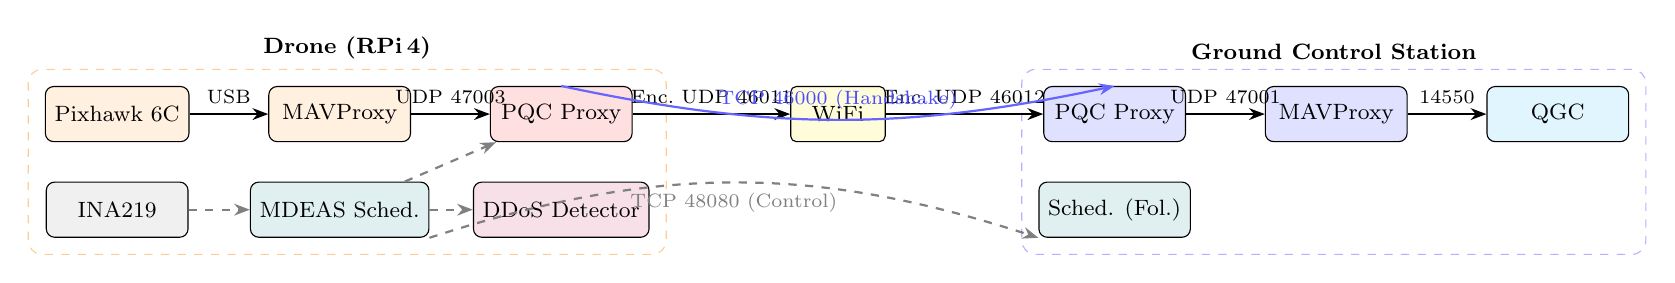
\begin{tikzpicture}[
        node distance=0.8cm and 1.0cm,
        box/.style={draw, rounded corners=3pt, minimum height=0.7cm, minimum width=1.8cm, font=\footnotesize, fill=#1!12, align=center},
        box/.default=blue,
        arr/.style={-{Stealth[length=2mm]}, thick},
        lbl/.style={font=\scriptsize, midway, align=center},
        dasharr/.style={-{Stealth[length=2mm]}, thick, dashed, gray},
        groupbox/.style={draw, dashed, rounded corners=5pt, inner sep=6pt, #1},
    ]
    % ---- DRONE SIDE ----
    \node[box=orange] (pixhawk) {Pixhawk 6C};
    \node[box=orange, right=of pixhawk] (mavproxy-d) {MAVProxy};
    \node[box=red, right=of mavproxy-d] (proxy-d) {PQC Proxy};
    \node[box=purple, below=0.5cm of proxy-d] (detector) {DDoS Detector};
    \node[box=teal, below=0.5cm of mavproxy-d] (scheduler-d) {MDEAS Sched.};
    \node[box=gray, below=0.5cm of pixhawk] (ina219) {INA219};

    % Drone group
    \begin{scope}[on background layer]
    \node[groupbox=orange!40, fit=(pixhawk)(mavproxy-d)(proxy-d)(detector)(scheduler-d)(ina219), label={[font=\footnotesize\bfseries]above:Drone (RPi\,4)}] (drone-group) {};
    \end{scope}

    % ---- ENCRYPTED LINK ----
    \node[right=2.0cm of proxy-d, draw, fill=yellow!15, rounded corners=2pt, minimum height=0.7cm, minimum width=1.2cm, font=\footnotesize, align=center] (wifi) {WiFi};

    % ---- GCS SIDE ----
    \node[box=blue, right=2.0cm of wifi] (proxy-g) {PQC Proxy};
    \node[box=blue, right=of proxy-g] (mavproxy-g) {MAVProxy};
    \node[box=cyan, right=of mavproxy-g] (qgc) {QGC};
    \node[box=teal, below=0.5cm of proxy-g] (scheduler-g) {Sched. (Fol.)};

    % GCS group
    \begin{scope}[on background layer]
    \node[groupbox=blue!30, fit=(proxy-g)(mavproxy-g)(qgc)(scheduler-g), label={[font=\footnotesize\bfseries]above:Ground Control Station}] (gcs-group) {};
    \end{scope}

    % ---- ARROWS (Drone side) ----
    \draw[arr] (pixhawk) -- (mavproxy-d) node[lbl, above] {USB};
    \draw[arr] (mavproxy-d) -- (proxy-d) node[lbl, above] {UDP 47003};
    \draw[arr] (proxy-d) -- (wifi) node[lbl, above] {Enc.\ UDP 46011};
    \draw[dasharr] (scheduler-d) -- (proxy-d);
    \draw[dasharr] (scheduler-d) -- (detector);
    \draw[dasharr] (ina219) -- (scheduler-d);

    % ---- ARROWS (GCS side) ----
    \draw[arr] (wifi) -- (proxy-g) node[lbl, above] {Enc.\ UDP 46012};
    \draw[arr] (proxy-g) -- (mavproxy-g) node[lbl, above] {UDP 47001};
    \draw[arr] (mavproxy-g) -- (qgc) node[lbl, above] {14550};

    % ---- CONTROL CHANNEL ----
    \draw[dasharr, bend left=18] (scheduler-d.south east) to node[lbl, below, font=\scriptsize] {TCP 48080 (Control)} (scheduler-g.south west);

    % ---- HANDSHAKE ----
    \draw[arr, blue!60, bend right=12] (proxy-d.north) to node[lbl, above, font=\scriptsize, blue!70] {TCP 46000 (Handshake)} (proxy-g.north);

    \end{tikzpicture}%
    }% end resizebox
    \caption{End-to-end system architecture of \sys{}. Solid arrows show the data path; dashed arrows show control/monitoring relationships. The encrypted UDP channel carries AEAD-protected MAVLink packets; the TCP control channel carries scheduler commands, clock sync, and rekey negotiation.}
    \label{fig:arch-overview}
\end{figure*}

The drone-side companion computer (Raspberry Pi~4) runs MAVProxy~\cite{mavproxy} connected to the Pixhawk flight controller~\cite{pixhawk} via USB serial.
MAVProxy forwards telemetry to the PQC proxy over local UDP (ports 47003/47004).
The proxy encrypts each packet with the negotiated AEAD cipher using the session key derived during the PQC handshake, transmits it over WiFi on the encrypted UDP channel (ports 46011/46012), and the GCS-side proxy decrypts and delivers to the ground MAVProxy instance.
A TCP control channel (port 48080) carries scheduler commands, clock synchronisation, and rekey negotiation between the drone-driven scheduler and the GCS follower.

\subsection{Suite Registry Design}
\label{sec:suite-registry}

The suite registry is the combinatorial backbone of \sys{}.
Each suite is a triple $(\mathrm{KEM}, \mathrm{SIG}, \mathrm{AEAD})$ where the KEM and SIG must share the same NIST security level.
We include algorithms from three KEM families and three signature families at three NIST levels, crossed with three AEAD ciphers.

\textbf{NIST Level Mapping.}
\begin{itemize}[noitemsep]
    \item \textbf{L1} ($\approx$AES-128 security): ML-KEM-512, HQC-128, Classic-McEliece-348864, ML-DSA-44\footnote{ML-DSA-44 is classified as NIST Level~2 in FIPS~204; we map it to L1 for practical pairing with L1 KEMs following the rationale that L2 exceeds L1 by a small margin.}, Falcon-512, SPHINCS$^+$-128s.
    \item \textbf{L3} ($\approx$AES-192 security): ML-KEM-768, HQC-192, Classic-McEliece-460896, ML-DSA-65, SPHINCS$^+$-192s.
    \item \textbf{L5} ($\approx$AES-256 security): ML-KEM-1024, HQC-256, Classic-McEliece-8192128, ML-DSA-87, Falcon-1024, SPHINCS$^+$-256s.
\end{itemize}

The level-consistent pairing produces:
\begin{equation}
\label{eq:suite-count}
    |\mathcal{S}| = \underbrace{(3 \times 3)}_{\text{L1}} + \underbrace{(3 \times 2)}_{\text{L3}} + \underbrace{(3 \times 3)}_{\text{L5}} = 24
\end{equation}
KEM$\times$SIG pairs ($\text{L3}$ has no Falcon variant), each crossed with 3 AEADs:
\begin{equation}
    N_{\text{suites}} = 24 \times 3 = 72
\end{equation}

Each suite is assigned a canonical identifier of the form \texttt{cs-\{kem\}-\{aead\}-\{sig\}} (e.g., \texttt{cs-mlkem768-aesgcm-mldsa65}).

Table~\ref{tab:kem-params} summarises the KEM parameters, and Table~\ref{tab:sig-params} summarises the signature parameters.

\begin{table}[t]
\centering
\caption{KEM Algorithm Parameters (from liboqs 0.14.0)}
\label{tab:kem-params}
\small
\begin{tabular}{@{}llrrr@{}}
\toprule
\textbf{Algorithm} & \textbf{Level} & \textbf{PK (B)} & \textbf{CT (B)} & \textbf{SS (B)} \\
\midrule
ML-KEM-512 & L1 & 800 & 768 & 32 \\
ML-KEM-768 & L3 & 1\,184 & 1\,088 & 32 \\
ML-KEM-1024 & L5 & 1\,568 & 1\,568 & 32 \\
HQC-128 & L1 & 2\,249 & 4\,433 & 64 \\
HQC-192 & L3 & 4\,522 & 9\,026 & 64 \\
HQC-256 & L5 & 7\,245 & 14\,469 & 64 \\
McEliece-348864 & L1 & 261\,120 & 96 & 32 \\
McEliece-460896 & L3 & 524\,160 & 156 & 32 \\
McEliece-8192128 & L5 & 1\,357\,824 & 208 & 32 \\
\bottomrule
\end{tabular}
\end{table}

\begin{table}[t]
\centering
\caption{Signature Algorithm Parameters (from liboqs 0.14.0)}
\label{tab:sig-params}
\small
\begin{tabular}{@{}llrrr@{}}
\toprule
\textbf{Algorithm} & \textbf{Level} & \textbf{PK (B)} & \textbf{SK (B)} & \textbf{Sig (B)} \\
\midrule
ML-DSA-44 & L1 & 1\,312 & 2\,560 & 2\,420 \\
ML-DSA-65 & L3 & 1\,952 & 4\,032 & 3\,309 \\
ML-DSA-87 & L5 & 2\,592 & 4\,896 & 4\,627 \\
Falcon-512 & L1 & 897 & 1\,281 & $\leq$666 \\
Falcon-1024 & L5 & 1\,793 & 2\,305 & $\leq$1\,280 \\
SPHINCS$^+$-128s & L1 & 32 & 64 & 7\,856 \\
SPHINCS$^+$-192s & L3 & 48 & 96 & 16\,224 \\
SPHINCS$^+$-256s & L5 & 64 & 128 & 29\,792 \\
\bottomrule
\end{tabular}
\end{table}

\subsection{KEM-Based Key Establishment}

The handshake uses a two-message protocol over TCP (port 46000):

\textbf{Message 1: ServerHello} (GCS $\to$ Drone).
The GCS generates an ephemeral KEM key pair $(pk_{\mathrm{kem}}, sk_{\mathrm{kem}}) \gets \mathrm{KEM.KeyGen}()$, a random 8-byte session identifier $\mathit{sid}$, and a random 8-byte challenge $c$.
It constructs the transcript:
\begin{equation}
\label{eq:transcript}
\begin{split}
    T = v \mathbin\| \texttt{pq-drone-gcs:v1} \mathbin\| \mathit{sid} \\
    \mathbin\| \mathrm{kem\_name} \mathbin\| \mathrm{sig\_name} \mathbin\| pk_{\mathrm{kem}} \mathbin\| c
\end{split}
\end{equation}
where $v$ is the frozen wire version byte.
The GCS signs the transcript:
$\sigma_{\mathrm{gcs}} \gets \mathrm{SIG.Sign}(sk_{\mathrm{gcs}}, T)$
and sends the length-prefixed wire message containing all fields plus $\sigma_{\mathrm{gcs}}$.

\textbf{Message 2: ClientReply} (Drone $\to$ GCS).
The drone verifies $\sigma_{\mathrm{gcs}}$ using the pre-distributed GCS public key, checks that the negotiated algorithms match the expected suite (anti-downgrade), and computes:
\begin{equation}
    (\mathit{ct}, K) \gets \mathrm{KEM.Encaps}(pk_{\mathrm{kem}})
\end{equation}
where $K$ is the shared secret.
It also computes an HMAC authentication tag over the entire ServerHello wire:
\begin{equation}
    \tau = \mathrm{HMAC\text{-}SHA256}(\mathit{PSK}, \mathit{ServerHello}_{\mathrm{wire}})
\end{equation}
and sends $(ct, \tau)$.

\textbf{Key Derivation.}
Both sides derive directional transport keys using HKDF-SHA256~\cite{rfc5869}:
\begin{equation}
\label{eq:hkdf}
    (k_{d \to g} \mathbin\| k_{g \to d}) = \mathrm{HKDF\text{-}SHA256}(K, s, \mathit{info}, 64)
\end{equation}
where the salt $s = \texttt{``pq\text{-}drone\text{-}gcs|hkdf|v1''}$ and $\mathit{info} = \texttt{``pq\text{-}drone\text{-}gcs:kdf:v1|''} \mathbin\| \mathit{sid} \mathbin\| \mathrm{kem\_name} \mathbin\| \mathrm{sig\_name}$.
The shared secret $K$ is zeroed immediately after derivation, following the WireGuard pattern.

Fig.~\ref{fig:handshake} illustrates the complete two-message handshake.

\begin{figure}[t]
    \centering
    \resizebox{\columnwidth}{!}{%
    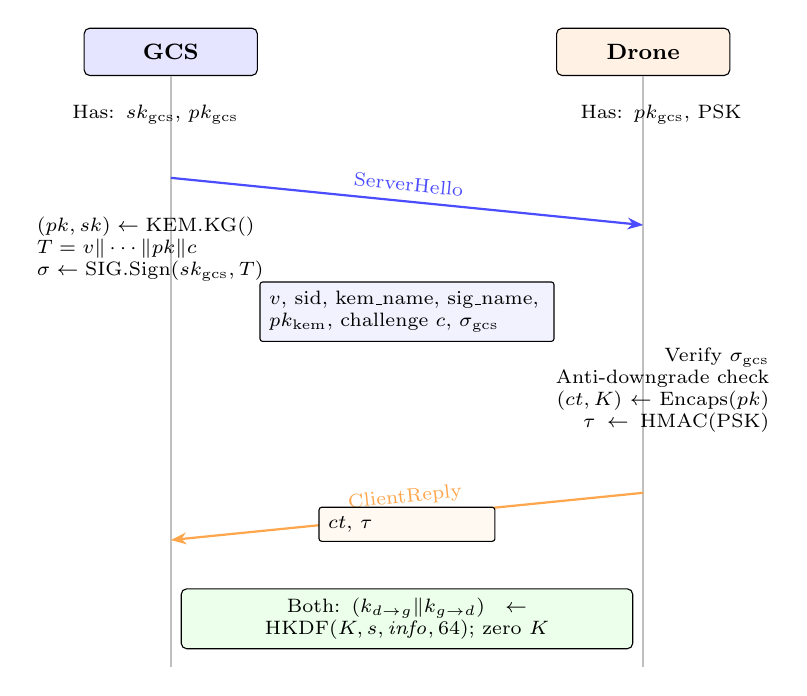
\begin{tikzpicture}[
        font=\footnotesize,
        entity/.style={draw, fill=#1!10, minimum width=2.2cm, minimum height=0.6cm, rounded corners=2pt, font=\footnotesize\bfseries},
        entity/.default=blue,
        msg/.style={-{Stealth[length=2mm]}, thick},
        note/.style={font=\scriptsize, text width=3cm, align=left},
    ]
    % Entities
    \node[entity=blue] (gcs) at (0,0) {GCS};
    \node[entity=orange] (drone) at (6,0) {Drone};

    % Lifelines
    \draw[thick, gray!50] (gcs.south) -- ++(0,-7.5);
    \draw[thick, gray!50] (drone.south) -- ++(0,-7.5);

    % Pre-state
    \node[note, text width=2.5cm] at (-0.0,-0.8) {\scriptsize Has: $sk_{\mathrm{gcs}}$, $pk_{\mathrm{gcs}}$};
    \node[note, text width=2.5cm, align=right] at (6.0,-0.8) {\scriptsize Has: $pk_{\mathrm{gcs}}$, PSK};

    % Message 1: ServerHello
    \draw[msg, blue!70] (0,-1.6) -- (6,-2.2) node[midway, above, sloped, font=\scriptsize] {ServerHello};
    \node[note] at (-0.2,-2.5) {
        $(pk,sk) \gets \mathrm{KEM.KG}()$\\
        $T = v \| \cdots \| pk \| c$\\
        $\sigma \gets \mathrm{SIG.Sign}(sk_\mathrm{gcs}, T)$
    };

    % Message 1 contents
    \node[draw, fill=blue!5, rounded corners=1pt, font=\scriptsize, text width=3.5cm, align=left] at (3,-3.3) {
        $v$, sid, kem\_name, sig\_name,\\
        $pk_{\mathrm{kem}}$, challenge $c$, $\sigma_{\mathrm{gcs}}$
    };

    % Drone processing
    \node[note, align=right, text width=2.8cm] at (6.2,-4.3) {
        Verify $\sigma_{\mathrm{gcs}}$\\
        Anti-downgrade check\\
        $(ct, K) \gets \mathrm{Encaps}(pk)$\\
        $\tau \gets \mathrm{HMAC}(\mathrm{PSK})$
    };

    % Message 2: ClientReply
    \draw[msg, orange!70] (6,-5.6) -- (0,-6.2) node[midway, above, sloped, font=\scriptsize] {ClientReply};
    \node[draw, fill=orange!5, rounded corners=1pt, font=\scriptsize, text width=2cm, align=left] at (3,-6.0) {
        $ct$, $\tau$
    };

    % Key derivation (both sides)
    \node[draw, fill=green!8, rounded corners=2pt, font=\scriptsize, text width=5.5cm, align=center] at (3,-7.2) {
        Both: $(k_{d\to g} \| k_{g\to d}) \gets \mathrm{HKDF}(K, s, \mathit{info}, 64)$; zero $K$
    };

    \end{tikzpicture}%
    }% end resizebox
    \caption{Two-message post-quantum handshake protocol. The GCS authenticates via digital signature; the drone authenticates via HMAC over PSK. Both sides derive directional transport keys from the KEM shared secret.}
    \label{fig:handshake}
\end{figure}

\subsection{AEAD Data-Plane Framing}

Each plaintext MAVLink packet is encrypted under the negotiated AEAD cipher.
The wire format is:
\begin{equation}
    \mathit{frame} = \underbrace{H}_{\text{22\,B header}} \mathbin\| \mathrm{AEAD.Enc}(k, \mathit{iv}, \mathit{pt}, H)
\end{equation}

The 22-byte header $H$ is structured as:
\[
H = (v, \mathit{kem\_id}, \mathit{kem\_p}, \mathit{sig\_id}, \mathit{sig\_p}, \mathit{sid}^{8}, \mathit{seq}^{8}, \mathit{epoch})
\]
and is bound as associated authenticated data (AAD) to the AEAD operation.
The 12-byte initialisation vector is deterministically constructed from the epoch byte and sequence number, avoiding IV transmission and saving 12~bytes per packet:
\begin{equation}
    \mathit{iv} = \mathit{epoch} \mathbin\| \mathit{seq}_{11\text{B}}
\end{equation}

Replay protection follows the WireGuard/RFC~6479 sliding-window approach with a configurable window $W$ (default 1024).
The implementation uses a split \emph{check/commit} pattern: the replay window is checked \emph{before} AEAD decryption and committed \emph{after} successful authentication, preventing a malicious packet from shifting the window without valid authentication.

Fig.~\ref{fig:aead-wire} illustrates the complete AEAD wire format.

\begin{figure}[!b]
    \centering
    \resizebox{\columnwidth}{!}{%
    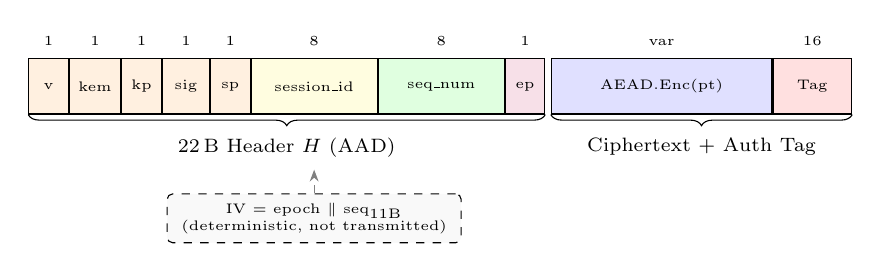
\begin{tikzpicture}[
        font=\footnotesize,
        field/.style={draw, minimum height=0.7cm, anchor=west, fill=#1!12, font=\scriptsize, align=center},
        field/.default=blue,
        brace/.style={decorate, decoration={brace, amplitude=4pt, mirror}},
        braceup/.style={decorate, decoration={brace, amplitude=4pt}},
        lbl/.style={font=\tiny, align=center},
    ]
    % ---- 22-byte Header (AAD) ----
    \node[field=orange, minimum width=0.5cm] (v) at (0,0) {\tiny v};
    \node[field=orange, minimum width=0.6cm, right=0pt of v] (kemid) {\tiny kem};
    \node[field=orange, minimum width=0.5cm, right=0pt of kemid] (kemp) {\tiny kp};
    \node[field=orange, minimum width=0.6cm, right=0pt of kemp] (sigid) {\tiny sig};
    \node[field=orange, minimum width=0.5cm, right=0pt of sigid] (sigp) {\tiny sp};
    \node[field=yellow, minimum width=1.6cm, right=0pt of sigp] (sid) {\tiny session\_id};
    \node[field=green, minimum width=1.6cm, right=0pt of sid] (seq) {\tiny seq\_num};
    \node[field=purple, minimum width=0.5cm, right=0pt of seq] (epoch) {\tiny ep};

    % ---- Ciphertext + Tag ----
    \node[field=blue, minimum width=2.8cm, right=2pt of epoch] (ct) {\tiny AEAD.Enc(pt)};
    \node[field=red, minimum width=1.0cm, right=0pt of ct] (tag) {\tiny Tag};

    % ---- Byte counts ----
    \node[lbl, above=1pt of v] {1};
    \node[lbl, above=1pt of kemid] {1};
    \node[lbl, above=1pt of kemp] {1};
    \node[lbl, above=1pt of sigid] {1};
    \node[lbl, above=1pt of sigp] {1};
    \node[lbl, above=1pt of sid] {8};
    \node[lbl, above=1pt of seq] {8};
    \node[lbl, above=1pt of epoch] {1};
    \node[lbl, above=1pt of ct] {var};
    \node[lbl, above=1pt of tag] {16};

    % ---- Braces ----
    \draw[brace] (v.south west) -- (epoch.south east) node[midway, below=5pt, font=\scriptsize] {22\,B Header $H$ (AAD)};
    \draw[brace] (ct.south west) -- (tag.south east) node[midway, below=5pt, font=\scriptsize] {Ciphertext + Auth Tag};

    % ---- IV derivation note ----
    \node[draw, dashed, rounded corners=2pt, fill=gray!5, font=\tiny, text width=3.5cm, align=center, below=1.0cm of sid] (ivnote) {IV = epoch $\|$ seq$_{11\text{B}}$ \\ (deterministic, not transmitted)};
    \draw[-{Stealth[length=1.5mm]}, dashed, gray] (ivnote.north) -- ++(0,0.3);
    \end{tikzpicture}%
    }% end resizebox
    \caption{AEAD wire format. The 22-byte header serves as AAD bound to the AEAD encryption. The IV is deterministically derived from epoch and sequence number, eliminating IV transmission overhead.}
    \label{fig:aead-wire}
\end{figure}

\subsection{Rekey Protocol}

Two rekey modes are supported:

\textbf{Cold Restart.}
The proxy process is terminated, a new handshake is performed with the target suite, and a fresh proxy is started.
This mode provides the strongest isolation between suites, as no key material persists across the restart boundary.
It incurs a brief blackout ($\sim$\SI{2}{\second}) during transition.

\textbf{In-Band Rekey.}
The proxy remains running; the scheduler sends a \texttt{prepare\_rekey} control message (packet type 0x02) through the encrypted channel.
Both sides execute a new handshake on the TCP port (serialised with a lock to avoid port conflicts), atomically swap the AEAD \texttt{Sender}/\texttt{Receiver} objects, and zero the old key material.
This minimises blackout but requires careful coordination via a two-phase commit protocol:

\begin{enumerate}[noitemsep]
    \item Coordinator $\to$ Follower: \texttt{prepare\_rekey($\mathit{suite}$, $\mathit{rid}$)}
    \item Follower $\to$ Coordinator: \texttt{prepare\_ok($\mathit{rid}$)} or \texttt{prepare\_fail}
    \item Coordinator $\to$ Follower: \texttt{commit\_rekey($\mathit{suite}$, $\mathit{rid}$)}
    \item Both execute handshake $\to$ atomic cipher swap
\end{enumerate}

Fig.~\ref{fig:rekey-flow} illustrates both rekey modes.

\begin{figure}[!b]
    \centering
    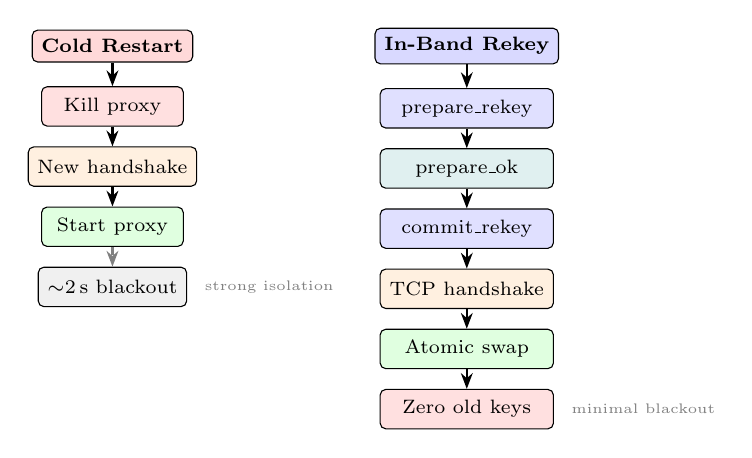
\begin{tikzpicture}[
        font=\footnotesize,
        box/.style={draw, rounded corners=2pt, minimum height=0.5cm, minimum width=1.8cm, fill=#1!12, font=\scriptsize, align=center},
        box/.default=blue,
        arr/.style={-{Stealth[length=2mm]}, thick},
        darr/.style={-{Stealth[length=2mm]}, thick, dashed},
        phase/.style={font=\scriptsize\bfseries, fill=#1!15, draw, rounded corners=2pt, minimum width=2cm, minimum height=0.4cm},
        phase/.default=gray,
    ]
    % ---- Cold Restart (left) ----
    \node[phase=red] (cr-title) at (0,0) {Cold Restart};
    \node[box=red, below=0.3cm of cr-title] (cr1) {Kill proxy};
    \node[box=orange, below=0.25cm of cr1] (cr2) {New handshake};
    \node[box=green, below=0.25cm of cr2] (cr3) {Start proxy};
    \node[box=gray, below=0.25cm of cr3] (cr4) {$\sim$2\,s blackout};

    \draw[arr] (cr-title) -- (cr1);
    \draw[arr] (cr1) -- (cr2);
    \draw[arr] (cr2) -- (cr3);
    \draw[darr, gray] (cr3) -- (cr4);

    % ---- In-Band Rekey (right) ----
    \node[phase=blue] (ib-title) at (4.5,0) {In-Band Rekey};

    \node[box=blue, below=0.3cm of ib-title, minimum width=2.2cm] (ib1) {prepare\_rekey};
    \node[box=teal, below=0.25cm of ib1, minimum width=2.2cm] (ib2) {prepare\_ok};
    \node[box=blue, below=0.25cm of ib2, minimum width=2.2cm] (ib3) {commit\_rekey};
    \node[box=orange, below=0.25cm of ib3, minimum width=2.2cm] (ib4) {TCP handshake};
    \node[box=green, below=0.25cm of ib4, minimum width=2.2cm] (ib5) {Atomic swap};
    \node[box=red, below=0.25cm of ib5, minimum width=2.2cm] (ib6) {Zero old keys};

    \draw[arr] (ib-title) -- (ib1);
    \draw[arr] (ib1) -- (ib2);
    \draw[arr] (ib2) -- (ib3);
    \draw[arr] (ib3) -- (ib4);
    \draw[arr] (ib4) -- (ib5);
    \draw[arr] (ib5) -- (ib6);

    % ---- Annotations ----
    \node[font=\tiny, text=gray, right=0.1cm of cr4] {strong isolation};
    \node[font=\tiny, text=gray, right=0.1cm of ib6] {minimal blackout};
    \end{tikzpicture}
    \caption{Rekey protocol modes. Cold restart (left) provides full key isolation with $\sim$2\,s blackout. In-band rekey (right) uses a two-phase commit to atomically swap cipher state with minimal disruption.}
    \label{fig:rekey-flow}
\end{figure}

The rekey overhead fraction for a session of duration $R$ with handshake time $T_{\mathrm{hs}}$ is:
\begin{equation}
\label{eq:rekey-overhead}
    \Phi(R) = \frac{T_{\mathrm{hs}}}{R + T_{\mathrm{hs}}}
\end{equation}

For the default suite (ML-KEM-768 + ML-DSA-65, $T_{\mathrm{hs}} = \SI{17.811}{\milli\second}$) with a 60-second rekey interval, $\Phi = 0.030\%$.

\subsection{DDoS Detection Pipeline}

The DDoS detection pipeline runs on the companion computer alongside the PQC proxy.
Two detection tiers are available:

\textbf{XGBoost Detector.}
A gradient-boosted tree model operating on 54 extracted features per traffic window.
Inference takes {\raise.17ex\hbox{$\scriptstyle\sim$}}\SI{7}{\milli\second} per window.
In this manuscript version, XGBoost overhead is treated as a configured policy prior rather than a measured cross-suite thermal/power delta, because canonical power telemetry is unavailable.

\textbf{Time Series Transformer (TST) Detector.}
A Transformer-based intrusion detection model operating on 46 features.
Inference takes {\raise.17ex\hbox{$\scriptstyle\sim$}}\SI{11}{\milli\second} per window.
Likewise, TST overhead is handled through configured safety margins in the scheduler model.

The scheduler maintains conservative safety margins for detector overhead (\SI{0.95}{\watt}/\SI{4.8}{\celsius} for XGBoost, \SI{1.97}{\watt}/\SI{10.7}{\celsius} for TST) in its \texttt{DetectorOverhead} configuration, ensuring headroom for worst-case conditions.

Fig.~\ref{fig:ddos-pipeline} illustrates the two-tier detection pipeline architecture.

\begin{figure}[!tb]
    \centering
    \resizebox{\columnwidth}{!}{%
    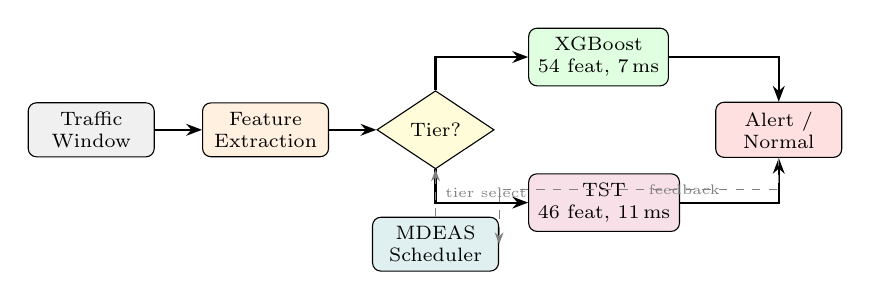
\begin{tikzpicture}[
        font=\footnotesize,
        box/.style={draw, rounded corners=3pt, minimum height=0.6cm, minimum width=1.6cm, fill=#1!12, font=\scriptsize, align=center},
        box/.default=blue,
        arr/.style={-{Stealth[length=2mm]}, thick},
        darr/.style={-{Stealth[length=1.5mm]}, dashed, gray},
    ]
    % Input
    \node[box=gray] (input) at (0,0) {Traffic\\Window};

    % Feature extraction
    \node[box=orange, right=0.6cm of input] (feat) {Feature\\Extraction};

    % Tier selection (switch)
    \node[draw, diamond, aspect=1.5, fill=yellow!15, font=\scriptsize, right=0.6cm of feat, minimum width=1cm] (switch) {Tier?};

    % XGBoost path
    \node[box=green, above right=0.3cm and 0.8cm of switch] (xgb) {XGBoost\\54 feat, 7\,ms};

    % TST path
    \node[box=purple, below right=0.3cm and 0.8cm of switch] (tst) {TST\\46 feat, 11\,ms};

    % Output
    \node[box=red, right=2.8cm of switch] (alert) {Alert /\\Normal};

    % Scheduler feedback
    \node[box=teal, below=0.6cm of switch] (sched) {MDEAS\\Scheduler};

    % Arrows
    \draw[arr] (input) -- (feat);
    \draw[arr] (feat) -- (switch);
    \draw[arr] (switch) |- (xgb) node[midway, above, font=\tiny] {};
    \draw[arr] (switch) |- (tst);
    \draw[arr] (xgb) -| (alert);
    \draw[arr] (tst) -| (alert);
    \draw[darr] (sched) -- (switch) node[midway, right, font=\tiny] {tier select};
    \draw[darr] (alert.south) -- ++(0,-0.4) -| (sched.east) node[near start, right, font=\tiny] {feedback};
    \end{tikzpicture}%
    }% end resizebox
    \caption{Two-tier DDoS detection pipeline. The MDEAS scheduler selects the active detector tier based on thermal/compute budget. Only one detector operates at a time; detection alerts feed back into scheduler decisions.}
    \label{fig:ddos-pipeline}
\end{figure}

Only one detector runs at any time (the companion computer lacks resources for concurrent operation).
The scheduler manages transitions between detector levels using the same process-group lifecycle management as proxy processes.

\subsection{Three-Axis Expert Scheduler (MDEAS)}
\label{sec:scheduler}

The Measurement-Driven Energy-Aware Scheduler (MDEAS) treats crypto agility as a joint optimisation problem over three axes:

\textbf{Axis 1 --- AEAD Selection} (data-plane, per-packet cost).
Selects among \{ChaCha20-Poly1305, AES-256-GCM, Ascon-128a\} based on measured per-packet encrypt/decrypt latency, temperature, and CPU utilisation.
The AEAD cost profile is maintained as an exponentially weighted moving average (EWMA) with $\alpha = 0.2$ (steady state) and pre-seeded from benchmark data (Benchmark-Seeded Initialisation):
\begin{equation}
\label{eq:ewma}
    \hat{C}_{n+1} = \alpha \cdot C_{\mathrm{obs}} + (1 - \alpha) \cdot \hat{C}_{n}
\end{equation}

\textbf{Axis 2 --- NIST Security Level} (control-plane, per-handshake cost).
Selects among \{L1, L3, L5\} with a fixed KEM+SIG pairing per level: L1$\to$(ML-KEM-512, ML-DSA-44), L3$\to$(ML-KEM-768, ML-DSA-65), L5$\to$(ML-KEM-1024, ML-DSA-87).

\textbf{Axis 3 --- DDoS Detection Level} (compute-plane, background cost).
Selects among \{None, XGBoost, TST\} based on threat indicators with awareness of detector overhead.

\textbf{Decision Cascade.}
The scheduler evaluates a 12-gate priority cascade at each tick:

\begin{enumerate}[noitemsep, label=\arabic*.]
    \item Telemetry stale ($> \SI{2}{\second}$) $\to$ HOLD
    \item DDoS detected (drop ratio $> 0.10$) $\to$ EMERGENCY
    \item Battery critical ($< \SI{14.0}{\volt}$) $\to$ EMERGENCY
    \item Temperature critical ($> \SI{80}{\celsius}$) $\to$ EMERGENCY
    \item Emergency active $\to$ kill detector
    \item Detector thermal ceiling exceeded $\to$ DOWNGRADE\_DETECTOR
    \item Predictive thermal crossing (\SI{60}{\second} extrapolation) $\to$ SWITCH\_AEAD
    \item Thermal/CPU stress $\to$ SWITCH\_AEAD (with break-even)
    \item AEAD recovery (stress subsided) $\to$ SWITCH\_AEAD
    \item Link degraded ($\text{gap}_{p95} > \SI{1}{\second}$) $\to$ DOWNGRADE\_LEVEL
    \item Stable conditions, proactive rekey due $\to$ REKEY
    \item Stable, upgrade hysteresis satisfied $\to$ UPGRADE
\end{enumerate}

\textbf{Break-Even Analysis.}
Before triggering an AEAD switch, the scheduler computes the break-even time:
\begin{equation}
\label{eq:break-even}
    t_{\mathrm{be}} = \frac{C_{\mathrm{rekey}}}{(\hat{C}_{\mathrm{cur}} - \hat{C}_{\mathrm{tgt}}) \cdot r_{\mathrm{pkt}} \cdot 2}
\end{equation}
where $C_{\mathrm{rekey}} = \SI{300}{\milli\second}$ is the handshake cost, $\hat{C}$ are the EWMA AEAD costs, and $r_{\mathrm{pkt}}$ is the packet rate.
The switch is executed only if $t_{\mathrm{be}} < \SI{30}{\second}$ (nominal) or $t_{\mathrm{be}} < \SI{15}{\second}$ (under stress).

\textbf{Hysteresis.}
Downgrade requires \SI{5}{\second} of sustained adverse conditions; upgrade requires \SI{30}{\second} of nominal conditions (tripled to \SI{90}{\second} when the vehicle is armed).
This prevents oscillation during transient load spikes.

\textbf{Cross-Axis Constraints.}
Not all axis combinations are permitted:
\begin{itemize}[noitemsep]
    \item Ascon-128a is forbidden with TST (combined overhead exceeds thermal budget).
    \item Classic McEliece is discouraged with TST (handshake length competes for CPU).
    \item Classic McEliece + SPHINCS$^+$ is forbidden at any detector level.
\end{itemize}

Fig.~\ref{fig:mdeas-cascade} illustrates the 12-gate decision cascade.

\begin{figure}[!b]
    \centering
    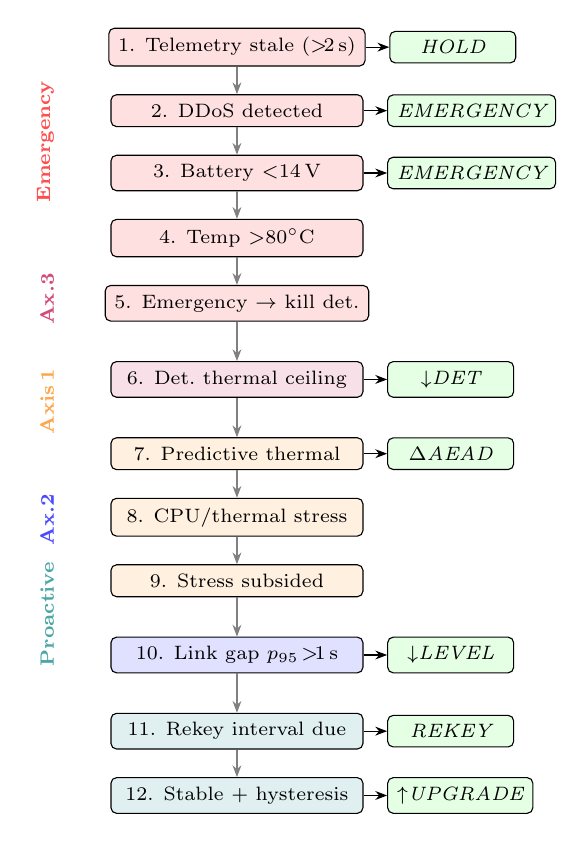
\begin{tikzpicture}[
        node distance=0.35cm,
        gate/.style={draw, rounded corners=2pt, minimum width=3.2cm, minimum height=0.38cm, font=\scriptsize, fill=#1!12, align=center},
        gate/.default=red,
        action/.style={draw, rounded corners=2pt, minimum width=1.6cm, minimum height=0.32cm, font=\scriptsize\itshape, fill=green!10, align=center},
        axislbl/.style={font=\scriptsize\bfseries, rotate=90, anchor=south},
        arr/.style={-{Stealth[length=1.5mm]}, thin},
    ]
    % Emergency gates
    \node[gate=red] (g1) {1. Telemetry stale ($>\!$2\,s)};
    \node[action, right=0.3cm of g1] (a1) {HOLD};
    \node[gate=red, below=of g1] (g2) {2. DDoS detected};
    \node[action, right=0.3cm of g2] (a2) {EMERGENCY};
    \node[gate=red, below=of g2] (g3) {3. Battery $<$14\,V};
    \node[gate=red, below=of g3] (g4) {4. Temp $>$80$^\circ$C};
    \node[action, right=0.3cm of g3] (a3) {EMERGENCY};
    \node[gate=red, below=of g4] (g5) {5. Emergency $\to$ kill det.};

    % Detector gate
    \node[gate=purple, below=0.5cm of g5] (g6) {6. Det.~thermal ceiling};
    \node[action, right=0.3cm of g6] (a6) {$\downarrow$DET};

    % AEAD gates
    \node[gate=orange, below=0.5cm of g6] (g7) {7. Predictive thermal};
    \node[action, right=0.3cm of g7] (a7) {$\Delta$AEAD};
    \node[gate=orange, below=of g7] (g8) {8. CPU/thermal stress};
    \node[gate=orange, below=of g8] (g9) {9. Stress subsided};

    % Level gate
    \node[gate=blue, below=0.5cm of g9] (g10) {10. Link gap $p_{95}\!>\!$1\,s};
    \node[action, right=0.3cm of g10] (a10) {$\downarrow$LEVEL};

    % Proactive gates
    \node[gate=teal, below=0.5cm of g10] (g11) {11. Rekey interval due};
    \node[action, right=0.3cm of g11] (a11) {REKEY};
    \node[gate=teal, below=of g11] (g12) {12. Stable + hysteresis};
    \node[action, right=0.3cm of g12] (a12) {$\uparrow$UPGRADE};

    % Flow arrows
    \foreach \i/\j in {g1/g2, g2/g3, g3/g4, g4/g5, g5/g6, g6/g7, g7/g8, g8/g9, g9/g10, g10/g11, g11/g12} {
        \draw[arr, gray] (\i.south) -- (\j.north);
    }
    % Action arrows
    \draw[arr] (g1.east) -- (a1.west);
    \draw[arr] (g2.east) -- (a2.west);
    \draw[arr] (g3.east) -- (a3.west);
    \draw[arr] (g6.east) -- (a6.west);
    \draw[arr] (g7.east) -- (a7.west);
    \draw[arr] (g10.east) -- (a10.west);
    \draw[arr] (g11.east) -- (a11.west);
    \draw[arr] (g12.east) -- (a12.west);

    % Axis labels
    \node[axislbl, red!70] at (-2.2,-1.2) {Emergency};
    \node[axislbl, purple!70] at (-2.2,-3.2) {Ax.3};
    \node[axislbl, orange!70] at (-2.2,-4.5) {Axis\,1};
    \node[axislbl, blue!70] at (-2.2,-6.0) {Ax.2};
    \node[axislbl, teal!70] at (-2.2,-7.2) {Proactive};

    \end{tikzpicture}
    \caption{MDEAS 12-gate priority decision cascade. Gates are evaluated top-to-bottom; the first triggered gate determines the action. Emergency conditions (gates 1--5) take absolute priority; proactive upgrades (gate 12) require sustained stability.}
    \label{fig:mdeas-cascade}
\end{figure}

\FloatBarrier
% ============================================================
% V. EXPERIMENTAL SETUP
% ============================================================
\section{Experimental Setup}
\label{sec:setup}

\subsection{Hardware Platform}

\textbf{Drone Companion Computer.}
Raspberry Pi~4 Model~B Rev~1.5 with Broadcom BCM2711 SoC (4-core ARM Cortex-A72 at \SI{1.8}{\giga\hertz}), \SI{4}{\giga\byte} LPDDR4 RAM.
The CPU governor is locked to \texttt{performance} mode to eliminate frequency scaling artefacts.
Power is measured using a Texas Instruments INA219~\cite{ina219} bidirectional current/power monitor on the I$^2$C bus at address \texttt{0x40}, sampling at \SI{1}{\kilo\hertz} in high-speed ADC mode (BADC=0x0080, settle time \SI{0.4}{\milli\second}).
The shunt resistor is \SI{0.1}{\ohm}.
Voltage is read from register 0x02 (bits [15:3], LSB = \SI{4}{\milli\volt}); shunt voltage from register 0x01 (signed 16-bit, LSB = \SI{10}{\micro\volt}).
Energy is computed via trapezoidal integration over the power samples.
Temperature is read from \texttt{/sys/class/thermal/thermal\_zone0/temp}.

\textbf{Flight Controller.}
Pixhawk 6C Mini~\cite{pixhawk} running ArduPilot~\cite{ardupilot} (ArduCopter v4.5.7), connected to the companion computer via USB serial.
The flight controller provides real-time MAVLink telemetry including heartbeat, system status, battery voltage/current, attitude, and GPS position.

\textbf{Ground Control Station.}
Windows laptop running MAVProxy and QGroundControl, connected to the drone over WiFi.

Fig.~\ref{fig:testbed} shows the physical testbed connections.

\begin{figure}[!tb]
    \centering
    \resizebox{\columnwidth}{!}{%
    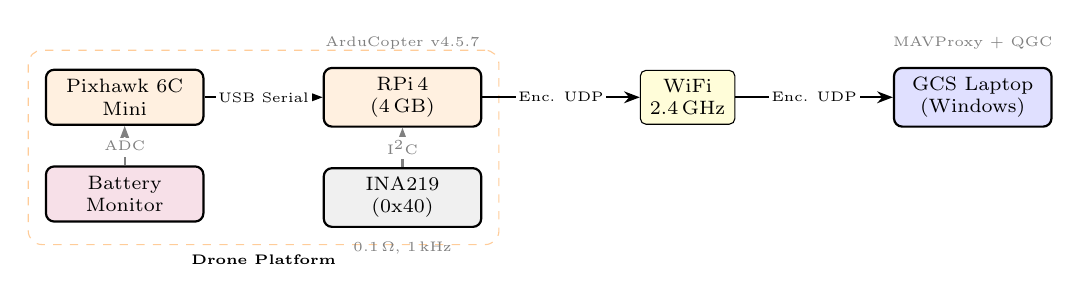
\begin{tikzpicture}[
        font=\footnotesize,
        hw/.style={draw, rounded corners=3pt, minimum height=0.7cm, minimum width=2.0cm, fill=#1!12, font=\scriptsize, align=center, thick},
        hw/.default=blue,
        conn/.style={-{Stealth[length=2mm]}, thick, #1},
        conn/.default=black,
        lbl/.style={font=\tiny, midway, fill=white, inner sep=1pt},
    ]
    % Drone side
    \node[hw=orange] (px) at (0,0) {Pixhawk 6C\\Mini};
    \node[hw=orange, right=1.5cm of px] (rpi) {RPi\,4\\(4\,GB)};
    \node[hw=gray, below=0.5cm of rpi] (ina) {INA219\\(0x40)};
    \node[hw=purple, below=0.5cm of px] (batt) {Battery\\Monitor};

    % Wireless
    \node[draw, fill=yellow!15, rounded corners=2pt, minimum width=1.2cm, minimum height=0.6cm, font=\scriptsize, align=center, right=2.0cm of rpi] (wifi) {WiFi\\2.4\,GHz};

    % GCS side
    \node[hw=blue, right=2.0cm of wifi] (laptop) {GCS Laptop\\(Windows)};

    % Connections
    \draw[conn] (px) -- (rpi) node[lbl] {USB Serial};
    \draw[conn, dashed, gray] (ina) -- (rpi) node[lbl] {I$^2$C};
    \draw[conn] (rpi) -- (wifi) node[lbl] {Enc. UDP};
    \draw[conn] (wifi) -- (laptop) node[lbl] {Enc. UDP};
    \draw[conn, dashed, gray] (batt) -- (px) node[lbl] {ADC};

    % Software labels
    \node[font=\tiny, text=gray, above=0.1cm of rpi] {ArduCopter v4.5.7};
    \node[font=\tiny, text=gray, above=0.1cm of laptop] {MAVProxy + QGC};
    \node[font=\tiny, text=gray, below=0.05cm of ina] {\SI{0.1}{\ohm}, \SI{1}{\kilo\hertz}};

    % Grouping
    \begin{scope}[on background layer]
    \node[draw, dashed, rounded corners=5pt, orange!40, fit=(px)(rpi)(ina)(batt), inner sep=6pt, label={[font=\tiny\bfseries]below:Drone Platform}] {};
    \end{scope}
    \end{tikzpicture}%
    }% end resizebox
    \caption{Experimental testbed hardware connections. The Pixhawk flight controller connects via USB serial to the RPi\,4 companion computer, which communicates with the GCS over encrypted WiFi. An INA219 sensor monitors power via I$^2$C.}
    \label{fig:testbed}
\end{figure}

\subsection{Software Stack}

\textbf{Cryptographic Libraries.}
\texttt{liboqs}~\cite{liboqs} version 0.14.0 (C library with ARM NEON optimisations), accessed via \texttt{liboqs-python}~\cite{oqspython}.
AEAD ciphers use the \texttt{cryptography}~\cite{cryptography-lib} Python package (AES-GCM, ChaCha20-Poly1305) and the \texttt{ascon}~\cite{ascon} Python package (Ascon-128a).

\textbf{Protocol Stack.}
MAVProxy~\cite{mavproxy} for MAVLink routing; \texttt{pymavlink} for protocol parsing and sequence tracking; \texttt{psutil} for system metrics; \texttt{smbus2} for INA219 register access.

\textbf{DDoS Detectors.}
XGBoost model ($\sim$\SI{33}{\mega\byte}, 54 features) and TST model (Transformer-based, 46 features), both running in dedicated Python virtual environments on the companion computer.

\textbf{Scheduling.}
The benchmarks use the \texttt{BenchmarkPolicy} with \SI{10}{\second} per suite, cold-restart mode, and sequential cycling through all 72 suites sorted by NIST level, then KEM, then signature.

\subsection{Benchmark Orchestration}

The benchmark is orchestrated by a PowerShell script (\texttt{run\_e2e\_benchmark.ps1}) that executes three phases:

\begin{enumerate}[noitemsep]
    \item \textbf{Phase~1 (Baseline):} All 72~suites with no DDoS detector.
    \item \textbf{Phase~2 (XGBoost):} All 72~suites with XGBoost detector active.
    \item \textbf{Phase~3 (TST):} All 72~suites with TST detector active.
\end{enumerate}

Each phase proceeds as follows: the GCS benchmark server starts locally; the drone benchmark scheduler is launched via SSH; for each suite, the drone orchestrator sends a \texttt{start\_proxy} command to the GCS, starts the local proxy, waits for the PQC handshake to complete, runs the MAVLink session for \SI{10}{\second}, collects metrics from both sides, and advances to the next suite.
Clock synchronisation between drone and GCS is performed every 10~suites using a Chronos-style NTP exchange over the TCP control channel.

A \SI{120}{\second} inter-phase cool-down allows thermal recovery between phases.

\subsection{Metrics Collection}

For each suite, a comprehensive JSON document is produced containing 18~metric categories (detailed in Section~\ref{sec:results}).
Timing is measured using \texttt{time.perf\_counter\_ns()} (nanosecond resolution).
Power samples are collected at \SI{1}{\kilo\hertz} throughout the session and integrated into per-suite energy values.
MAVLink integrity is monitored via a dedicated sniff port, tracking per-message-type counts, sequence gaps, heartbeat intervals, and RTT via COMMAND\_ACK and active PING probes.
For the canonical run used in this paper (\texttt{20260220\_full}), the power backend reported no valid samples; quantitative power/thermal comparisons are therefore excluded from the final analysis.

\FloatBarrier
% ============================================================
% VI. RESULTS AND ANALYSIS
% ============================================================
\section{Results and Analysis}
\label{sec:results}

We present results from the complete 72-suite benchmark across all three operational phases measured on the Raspberry Pi~4 platform.
All numbers are single-run observations from the production benchmark (run tag \texttt{20260220\_full}), measured under controlled lab conditions with CPU governor locked to \texttt{performance} mode.

\subsection{Reporting Scope and Data Provenance}

To keep claims auditable and semantically consistent, this section separates two evidence sources:
\begin{enumerate}[label=\textbf{R\arabic*}, leftmargin=2em]
    \item \textbf{Canonical suite results} from \texttt{benchmark\_full\_table\_20260220.csv}, used for handshake outcomes, success/failure counts, and cross-scenario comparisons.
    \item \textbf{Supporting primitive profiles} from \texttt{v2-1.8ghz}, used to interpret per-algorithm KEM/signature/AEAD cost trends.
\end{enumerate}

For this canonical run, all rows report \texttt{power\_status\_reason = no\_power\_samples (backend=none)}.
Accordingly, power/thermal conclusions are framed as policy-design priors or deferred to sensor-complete reruns, rather than presented as measured canonical outcomes.

\subsection{Key Results at a Glance}

Table~\ref{tab:key-takeaways} summarises the highest-impact verified outcomes for quick reviewer inspection before subsection-level detail.

\begin{table}[t]
\centering
\caption{Canonical Benchmark Takeaways (run tag \texttt{20260220\_full})}
\label{tab:key-takeaways}
\scriptsize
\begin{tabular}{@{}p{2.6cm}p{4.4cm}@{}}
\toprule
\textbf{Question} & \textbf{Verified Outcome} \\
\midrule
Suite sessions completed? & 213/216 successful (3 failures, all McEliece-460896 + SPHINCS$^+$-192s) \\
Fastest handshake? & ML-KEM-512 + Falcon-512 + AES-GCM at \SI{9.391}{\milli\second} \\
L3 operating point? & ML-KEM-768 + ML-DSA-65 + ChaCha20 at \SI{14.395}{\milli\second} \\
L5 lattice feasibility? & ML-KEM-1024 + ML-DSA-87 + AES-GCM at \SI{15.056}{\milli\second} \\
Crypto-layer integrity? & $d_{\text{replay}}=d_{\text{auth}}=d_{\text{header}}=0$ \\
Power/thermal status? & Unavailable (all rows: \texttt{no\_power\_samples}) \\
\bottomrule
\end{tabular}
\end{table}

\subsection{Individual KEM Benchmarks}

Table~\ref{tab:kem-timing} reports primitive-level KEM timing from the supporting benchmark pack (\texttt{v2-1.8ghz}).
These measurements isolate cryptographic operations and are used to interpret trends, while suite-level handshake claims in this section are taken from the canonical 72-suite run.

\begin{table}[t]
\centering
\caption{KEM Primitive Timing on RPi4 (v2-1.8ghz benchmark pack, INA219)}
\label{tab:kem-timing}
\small
\begin{tabular}{@{}lrrr@{}}
\toprule
\textbf{Algorithm} & \textbf{KeyGen} & \textbf{Encaps} & \textbf{Decaps} \\
 & (ms) & (ms) & (ms) \\
\midrule
ML-KEM-512 & 0.240 & 0.152 & 0.158 \\
ML-KEM-768 & 0.237 & 0.182 & 0.185 \\
ML-KEM-1024 & 0.273 & 0.216 & 0.231 \\
\midrule
HQC-128 & 22.3 & 44.7 & 73.4 \\
HQC-192 & 67.7 & 135.8 & 211.9 \\
HQC-256 & 124.4 & 250.2 & 392.6 \\
\midrule
McEliece-348864 & 351.0 & 0.47 & 56.0 \\
McEliece-460896 & 1\,281.4 & 0.87 & 89.6 \\
McEliece-8192128 & 9\,020.8 & 1.89 & 210.1 \\
\bottomrule
\end{tabular}
\end{table}

The ordering is clear: ML-KEM primitives are one to four orders of magnitude faster than HQC and Classic McEliece.
At the primitive level, ML-KEM-768 key generation is \SI{0.24}{\milli\second}, versus \SI{9021}{\milli\second} for Classic-McEliece-8192128.
At the suite level, the same pattern appears in canonical outcomes: lattice suites remain in the low-millisecond region, while heavy code-based combinations extend into seconds or tens of seconds.

\subsection{Signature Benchmarks}

Table~\ref{tab:sig-timing} reports primitive-level signature timing from the supporting benchmark pack (\texttt{v2-1.8ghz}).

\begin{table}[t]
\centering
\caption{Signature Primitive Timing on RPi4 (v2-1.8ghz benchmark pack)}
\label{tab:sig-timing}
\small
\begin{tabular}{@{}lrrr@{}}
\toprule
\textbf{Algorithm} & \textbf{Sign} & \textbf{Verify} & \textbf{Sig Size} \\
 & (ms) & (ms) & (B) \\
\midrule
ML-DSA-44 & 1.179 & 0.331 & 2\,420 \\
ML-DSA-65 & 1.633 & 0.484 & 3\,309 \\
ML-DSA-87 & 1.847 & 0.723 & 4\,627 \\
\midrule
Falcon-512 & 0.778 & 0.192 & 656 \\
Falcon-1024 & 1.452 & 0.280 & 1\,271 \\
\midrule
SPHINCS$^+$-128s & 1\,468.1 & 1.582 & 7\,856 \\
SPHINCS$^+$-192s & 2\,609.6 & 2.299 & 16\,224 \\
SPHINCS$^+$-256s & 2\,321.1 & 3.292 & 29\,792 \\
\bottomrule
\end{tabular}
\end{table}

Falcon-512 provides the fastest signing (\SI{0.78}{\milli\second}) and the smallest signatures (656~bytes).
ML-DSA stays in the same practical regime (sign under \SI{1.9}{\milli\second}, verify under \SI{0.8}{\milli\second}) while avoiding Falcon's floating-point sampling complexity.
SPHINCS$^+$ is the dominant signature cost driver: \SI{1468}{\milli\second} to \SI{2610}{\milli\second} signing with much larger artifacts, which directly amplifies handshake duration when paired with heavy KEMs.

\subsection{AEAD Data-Plane Cost}

Table~\ref{tab:aead-timing} reports per-packet AEAD cost for a typical MAVLink payload (\SI{\approx 280}{\byte}) from instrumented proxy profiling.

\begin{table}[t]
\centering
\caption{AEAD Per-Packet Cost on RPi4 (instrumented proxy profiling)}
\label{tab:aead-timing}
\small
\begin{tabular}{@{}lrr@{}}
\toprule
\textbf{AEAD} & \textbf{Encrypt (ns)} & \textbf{Decrypt (ns)} \\
\midrule
ChaCha20-Poly1305 & 71\,441 & 82\,504 \\
AES-256-GCM & 76\,341 & 83\,982 \\
Ascon-128a & 1\,374\,916 & 999\,440 \\
\bottomrule
\end{tabular}
\end{table}

ChaCha20-Poly1305 and AES-256-GCM are within 7\% on this platform, with ChaCha20 marginally faster on Cortex-A72.
Ascon-128a is substantially slower in the current software path (about $19\times$ encryption, $12\times$ decryption), so its operational use requires either lower packet-rate budgets or a native accelerated backend.

\subsection{Suite-Level Handshake Results}

Table~\ref{tab:suite-handshake} presents handshake latency for selected suites across all three NIST levels.

\begin{table}[t]
\centering
\caption{Selected Suite Handshake Latency (no-ddos, RPi4)}
\label{tab:suite-handshake}
\scriptsize
\begin{tabular}{@{}p{4.0cm}lr@{}}
\toprule
\textbf{Suite} & \textbf{Lvl} & \textbf{HS (ms)} \\
\midrule
ML-KEM-512 + Falcon-512 + AES-GCM & L1 & 9.391 \\
ML-KEM-512 + Falcon-512 + ChaCha20 & L1 & 9.948 \\
ML-KEM-768 + ML-DSA-65 + AES-GCM & L3 & 17.811 \\
ML-KEM-1024 + ML-DSA-87 + AES-GCM & L5 & 15.056 \\
HQC-128 + ML-DSA-44 + AES-GCM & L1 & 61.083 \\
HQC-256 + ML-DSA-87 + AES-GCM & L5 & 275.506 \\
McEliece-348864 + Falcon-512 + AES-GCM & L1 & 210.166 \\
McEliece-8192128 + ML-DSA-87 + AES-GCM & L5 & 1\,511.381 \\
McEliece-460896 + SPHINCS$^+$-192s + AES-GCM & L3 & 48\,268$^{\ddagger}$ \\
\bottomrule
\multicolumn{3}{@{}l}{\scriptsize $\ddagger$ \texttt{handshake\_ok\_both=False}; fails in all three scenarios.}
\end{tabular}
\end{table}

Fig.~\ref{fig:hs-selected} visualises the same selected-suite handshake results on a log scale to highlight the latency spread from lattice to heavy code/hash combinations.

\begin{figure}[t]
    \centering
    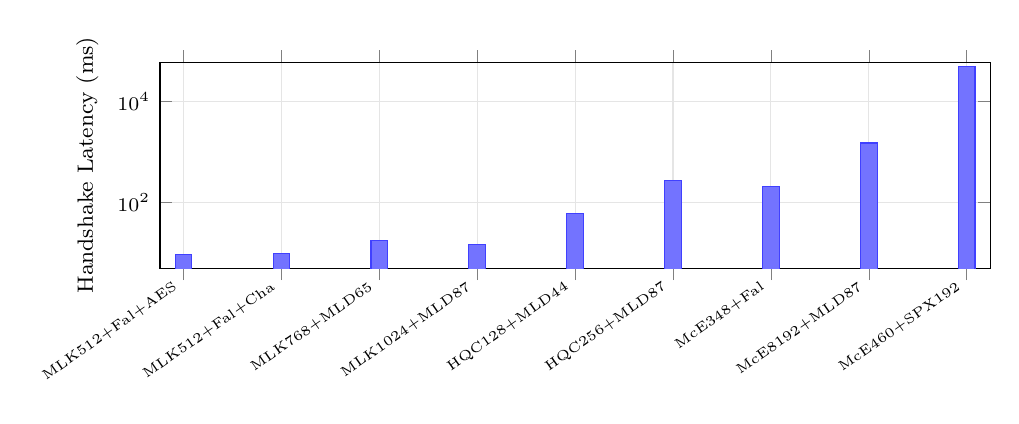
\begin{tikzpicture}
    \begin{axis}[
        ybar,
        bar width=6pt,
        width=\columnwidth,
        height=4.2cm,
        ylabel={Handshake Latency (ms)},
        ylabel style={font=\footnotesize},
        ymode=log,
        ymin=5,
        ymax=60000,
        symbolic x coords={MLK512+Fal+AES, MLK512+Fal+Cha, MLK768+MLD65, MLK1024+MLD87, HQC128+MLD44, HQC256+MLD87, McE348+Fal, McE8192+MLD87, McE460+SPX192},
        xtick=data,
        x tick label style={rotate=35, anchor=east, font=\tiny},
        tick label style={font=\scriptsize},
        grid=major,
        grid style={gray!20},
        enlarge x limits=0.03,
    ]
    \addplot[fill=blue!55, draw=blue!75] coordinates {
        (MLK512+Fal+AES,9.391)
        (MLK512+Fal+Cha,9.948)
        (MLK768+MLD65,17.811)
        (MLK1024+MLD87,15.056)
        (HQC128+MLD44,61.083)
        (HQC256+MLD87,275.506)
        (McE348+Fal,210.166)
        (McE8192+MLD87,1511.381)
        (McE460+SPX192,48268.476)
    };
    \end{axis}
    \end{tikzpicture}
    \caption{Selected suite handshake latency (no-ddos baseline, drone-side, log scale). Lattice-based suites remain sub-\SI{20}{\milli\second}, while the known failing McEliece+SPHINCS$^+$ combination is near \SI{48}{\second}.}
    \label{fig:hs-selected}
\end{figure}

Two operational points stand out.
First, the fastest validated suite (ML-KEM-512 + Falcon-512 + AES-GCM) completes at \SI{9.391}{\milli\second}, well inside MAVLink heartbeat timing.
Second, lattice Level-5 remains practical (ML-KEM-1024 + ML-DSA-87 at \SI{15.056}{\milli\second}).
At the opposite extreme, Classic-McEliece-460896 + SPHINCS$^+$-192s reaches \SI{48.268}{\second} and fails handshake validation.

Fig.~\ref{fig:aead-bar} compares per-packet AEAD costs.

\begin{figure}[t]
    \centering
    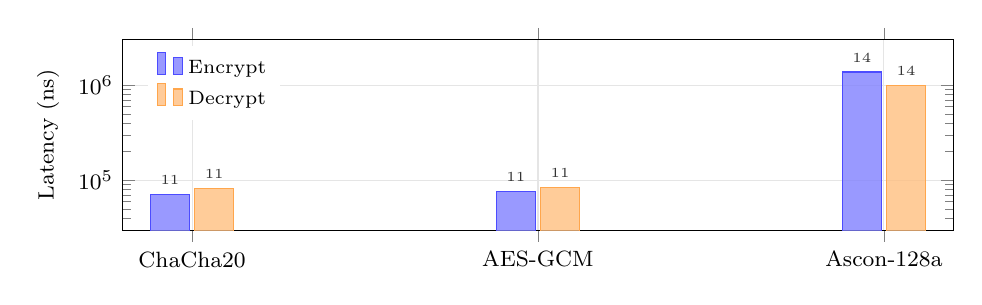
\begin{tikzpicture}
    \begin{axis}[
        ybar,
        bar width=14pt,
        width=\columnwidth,
        height=4cm,
        ylabel={Latency (ns)},
        ylabel style={font=\footnotesize},
        ymode=log,
        ymin=30000, ymax=3000000,
        symbolic x coords={ChaCha20, AES-GCM, Ascon-128a},
        xtick=data,
        tick label style={font=\footnotesize},
        legend style={at={(0.03,0.97)}, anchor=north west, font=\scriptsize, draw=none},
        grid=major,
        grid style={gray!20},
        nodes near coords,
        nodes near coords style={font=\tiny, above, rotate=0},
        every node near coord/.append style={/pgf/number format/.cd, fixed, precision=0, 1000 sep={\,}},
        every axis plot/.append style={fill opacity=0.8},
    ]
    \addplot[fill=blue!50, draw=blue!70] coordinates {
        (ChaCha20, 71441) (AES-GCM, 76341) (Ascon-128a, 1374916)
    };
    \addplot[fill=orange!50, draw=orange!70] coordinates {
        (ChaCha20, 82504) (AES-GCM, 83982) (Ascon-128a, 999440)
    };
    \legend{Encrypt, Decrypt}
    \end{axis}
    \end{tikzpicture}
    \caption{Per-packet AEAD cost comparison (log scale). ChaCha20-Poly1305 and AES-256-GCM are within 7\% of each other; Ascon-128a is 19$\times$ slower due to its pure-Python implementation.}
    \label{fig:aead-bar}
\end{figure}

\subsection{Rekey Overhead Analysis}

Using Equation~\ref{eq:rekey-overhead}, we compute the rekey overhead fraction for representative suites at the default \SI{60}{\second} rekey interval:

\begin{table}[t]
\centering
\caption{Rekey Overhead at \SI{60}{\second} Interval}
\label{tab:rekey-overhead}
\small
\begin{tabular}{@{}lr@{}}
\toprule
\textbf{Suite} & $\Phi(\SI{60}{\second})$ \\
\midrule
ML-KEM-512 + Falcon-512 + ChaCha20 & 0.018\% \\
ML-KEM-768 + ML-DSA-65 + AES-GCM & 0.030\% \\
HQC-256 + ML-DSA-87 + AES-GCM & 0.456\% \\
McEliece-8192128 + ML-DSA-87 + AES-GCM & 2.457\% \\
\bottomrule
\end{tabular}
\end{table}

ML-KEM-based suites incur negligible rekey overhead ($< 0.04\%$), enabling frequent rekeying for forward secrecy.
Heavy suites (Classic McEliece) should use longer rekey intervals or be reserved for initial establishment only.

\subsection{DDoS Impact on PQC Performance}

Table~\ref{tab:ddos-impact} compares the reference suite across baseline, XGBoost, and Transformer detector phases using canonical handshake measurements.

\begin{table}[t]
\centering
\caption{DDoS Detector Impact on ML-KEM-768 + ML-DSA-65 + AES-GCM}
\label{tab:ddos-impact}
\small
\begin{tabular}{@{}lrr@{}}
\toprule
\textbf{Phase} & \textbf{HS (ms)} & \textbf{Handshake Status} \\
\midrule
Baseline (no-ddos) & 17.811 & PASS \\
XGBoost detector & 61.661 & PASS \\
Transformer detector & 13.994 & PASS \\
\bottomrule
\end{tabular}
\end{table}

All three scenarios complete for this reference suite, but handshake latency varies across phases.
Given single-run conditions, we interpret this as runtime contention/noise rather than as a stable detector-overhead estimate.
Power and thermal deltas remain unavailable in the canonical run because all rows are marked \texttt{no\_power\_samples (backend=none)}.

\subsection{Packet Loss Analysis}

For the canonical run, crypto-layer packet loss is computed from authenticated tunnel drop counters:
\begin{equation}
\label{eq:crypto-drop-total}
d_{\text{crypto}} = d_{\text{replay}} + d_{\text{auth}} + d_{\text{header}}.
\end{equation}

Across all 213 successful sessions, aggregate values are
$d_{\text{replay}}=0$, $d_{\text{auth}}=0$, and $d_{\text{header}}=0$,
yielding zero crypto-layer loss for completed handshakes.
This metric intentionally excludes peer/session gating counters (e.g.,
\texttt{drop\_src\_addr}, \texttt{drop\_session\_epoch}) and MAV sequence-gap observations,
which are reported separately to avoid conflating transport rejection semantics with authenticated packet integrity loss.

\subsection{Power and Thermal Measurement Availability}

The benchmark framework includes INA219 and thermal instrumentation, but the canonical full run used for this paper contains no valid power samples (every row reports \texttt{no\_power\_samples (backend=none)}).
To avoid semantic drift, we therefore do not report quantitative cross-suite power, temperature, or energy comparisons in this version.
The scheduling discussion remains valid as a control-policy design analysis grounded in implementation logic, while quantitative thermal and power validation is left to a dedicated run with confirmed sensor capture.

\subsection{Scheduler Decision Impact}

The MDEAS scheduler responds to changing conditions along its three axes.
Table~\ref{tab:scheduler-scenarios} illustrates representative decisions.

\begin{table}[t]
\centering
\caption{MDEAS Scheduler Decision Scenarios}
\label{tab:scheduler-scenarios}
\small
\begin{tabular}{@{}p{3.5cm}p{4cm}@{}}
\toprule
\textbf{Condition} & \textbf{Action} \\
\midrule
Temp $> \SI{80}{\celsius}$ or Battery $< \SI{14}{\volt}$ & EMERGENCY: L1 + cheapest AEAD, kill detector \\
Temp crossing \SI{70}{\celsius} within \SI{60}{\second} & SWITCH\_AEAD to cooler cipher \\
DDoS detected (drop ratio $> 0.10$) & EMERGENCY: cheapest AEAD, lock \\
Detector thermal ceiling exceeded & DOWNGRADE\_DETECTOR \\
Link gap $p_{95} > \SI{1}{\second}$ & DOWNGRADE\_LEVEL \\
Stable for \SI{30}{\second} (armed: \SI{90}{\second}) & UPGRADE\_LEVEL \\
\bottomrule
\end{tabular}
\end{table}

The AEAD preference order on ARM Cortex-A72 is ChaCha20 $>$ AES-GCM $>$ Ascon-128a, reflecting the lack of hardware AES acceleration and the software overhead of Ascon.
The scheduler's seeded AEAD cost profiles (Table~\ref{tab:aead-seed}) drive switching decisions without requiring a learning warm-up:

\begin{table}[t]
\centering
\caption{AEAD Benchmark-Seeded Cost Profiles\protect\footnotemark}
\label{tab:aead-seed}
\small
\begin{tabular}{@{}lrrr@{}}
\toprule
\textbf{AEAD} & \textbf{Enc (ns)} & \textbf{Dec (ns)} & $\Delta T$ ($^\circ$C) \\
\midrule
ChaCha20-Poly1305 & 63\,500 & 70\,700 & 0.0 \\
AES-256-GCM & 66\,900 & 73\,600 & $-0.1$ \\
Ascon-128a & 1\,327\,100 & 960\,500 & $+1.5$ \\
\bottomrule
\end{tabular}
\end{table}
\footnotetext{Seed values (from \texttt{v2-1.8ghz} cold-start profiling) differ slightly from Table~\ref{tab:aead-timing} (instrumented proxy profiling) due to distinct measurement contexts: seed profiles capture isolated burst cost, while proxy profiling measures steady-state per-packet cost under live MAVLink traffic.}

\subsection{Graceful Degradation}

The scheduler implements graceful degradation through a tiered response.
When thermal stress is detected, the system first switches AEAD (Axis~1)---the cheapest corrective action affecting per-packet cost.
If stress persists, it downgrades the NIST level (Axis~2), reducing handshake complexity at the cost of security margin.
Finally, under sustained overload, it sheds the DDoS detector (Axis~3), freeing the largest configured compute budget in the policy model (\SI{0.95}--\SI{1.97}{\watt} equivalent).

This layered approach ensures that \emph{connectivity is always maintained}: the system never drops to unencrypted operation, but gracefully trades security margin and detection capability for thermal and energy sustainability.

Fig.~\ref{fig:degradation-ladder} visualises the three-tier degradation ladder.

\begin{figure}[!tb]
    \centering
    \resizebox{\columnwidth}{!}{%
    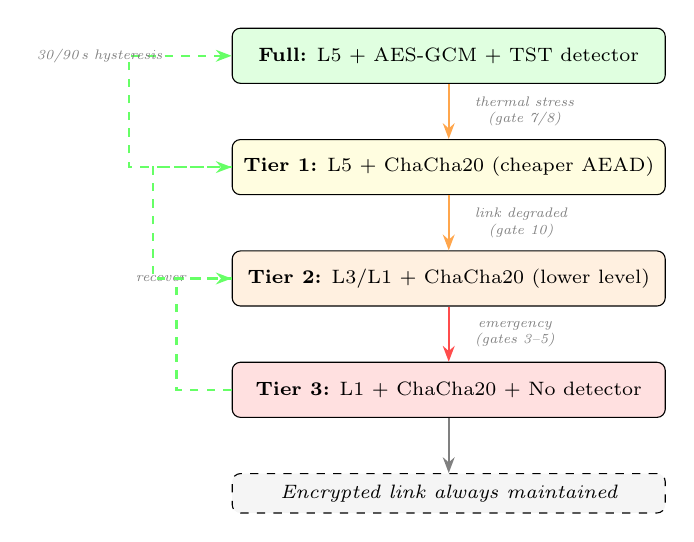
\begin{tikzpicture}[
        font=\footnotesize,
        tier/.style={draw, rounded corners=3pt, minimum height=0.7cm, minimum width=5.5cm, fill=#1!12, font=\scriptsize, align=center},
        tier/.default=green,
        arr/.style={-{Stealth[length=2mm]}, thick},
        trigger/.style={font=\tiny\itshape, text=gray, align=center},
    ]
    % Tier 0: Full capability
    \node[tier=green] (t0) at (0,0) {\textbf{Full:} L5 + AES-GCM + TST detector};

    % Tier 1: AEAD downgrade
    \node[tier=yellow, below=0.7cm of t0] (t1) {\textbf{Tier 1:} L5 + ChaCha20 (cheaper AEAD)};

    % Tier 2: Level downgrade
    \node[tier=orange, below=0.7cm of t1] (t2) {\textbf{Tier 2:} L3/L1 + ChaCha20 (lower level)};

    % Tier 3: Detector shed
    \node[tier=red, below=0.7cm of t2] (t3) {\textbf{Tier 3:} L1 + ChaCha20 + No detector};

    % Always-on floor
    \node[draw, dashed, rounded corners=3pt, minimum width=5.5cm, minimum height=0.5cm, fill=gray!8, font=\scriptsize\itshape, below=0.7cm of t3] (floor) {Encrypted link always maintained};

    % Arrows with triggers
    \draw[arr, orange!70] (t0) -- (t1) node[trigger, midway, right=0.2cm] {thermal stress\\(gate~7/8)};
    \draw[arr, orange!70] (t1) -- (t2) node[trigger, midway, right=0.2cm] {link degraded\\(gate~10)};
    \draw[arr, red!70] (t2) -- (t3) node[trigger, midway, right=0.2cm] {emergency\\(gates~3--5)};
    \draw[arr, gray] (t3) -- (floor);

    % Recovery arrows (left side)
    \draw[arr, green!60, dashed] (t3.west) -- ++(-0.7,0) |- (t2.west) node[trigger, near end, left=0.1cm] {\tiny recover};
    \draw[arr, green!60, dashed] (t2.west) -- ++(-1.0,0) |- (t1.west);
    \draw[arr, green!60, dashed] (t1.west) -- ++(-1.3,0) |- (t0.west) node[trigger, near end, left=0.1cm] {\tiny 30/90\,s hysteresis};
    \end{tikzpicture}%
    }% end resizebox
    \caption{Graceful degradation ladder. The system sheds capability in priority order: AEAD cost (cheapest), then security level, then detector shedding (most impactful). Recovery requires sustained stability with hysteresis to prevent oscillation.}
    \label{fig:degradation-ladder}
\end{figure}

\FloatBarrier
% ============================================================
% VII. DISCUSSION
% ============================================================
\section{Discussion}
\label{sec:discussion}

\subsection{Key Findings and Interpretation}

\textbf{ML-KEM-based suites provide the best latency envelope.}
Across the verified Pi~4 dataset, the fastest recorded handshake is \SI{9.391}{\milli\second} (\texttt{cs-mlkem512-aesgcm-falcon512}, no-DDoS).
Level-3 lattice configurations remain in the low-millisecond range in baseline conditions (for example, \texttt{cs-mlkem768-chacha20poly1305-mldsa65} at \SI{14.395}{\milli\second}), well below the MAVLink heartbeat interval (\SI{1}{\second}).

\textbf{Classic McEliece remains structurally conservative but operationally expensive.}
Classic McEliece's coding-theory security basis~\cite{mceliece} is attractive for diversity, but large public keys (261~KB to 1.3~MB) increase transfer and setup costs.
In the verified runs, \texttt{cs-classicmceliece460896-aesgcm-sphincs192s} is consistently near \SI{48}{\second} handshake duration and fails in all three scenarios, making it unsuitable for latency-critical flight loops.

\textbf{SPHINCS$^+$ overhead is dominated by signature size and verification cost.}
SPHINCS$^+$ (SLH-DSA)~\cite{sphincsplus} offers conservative hash-based security assumptions, but larger signatures increase both wire overhead and end-to-end handshake cost relative to Falcon and ML-DSA pairings.

\textbf{Detector management is the primary thermal-control lever in policy design.}
The scheduler's \texttt{DetectorOverhead} configuration budgets \SI{0.95}{\watt}/\SI{4.8}{\celsius} (XGBoost) and \SI{1.97}{\watt}/\SI{10.7}{\celsius} (TST) as conservative safety margins.
Because the canonical run lacks valid power telemetry, these values are treated as control-policy priors rather than measured outcomes for this dataset.

\subsection{Operational Implications}

For operational UAV deployments, these results suggest a simple policy hierarchy: select a low-latency lattice baseline for routine operation, reserve heavier suites for explicit high-assurance phases, and use detector-tier control as the primary emergency lever under thermal or battery stress.
This interpretation matches the scheduler design: AEAD changes as the cheapest frequent adjustment, security-level shifts as medium-cost control-plane adaptation, and detector shedding as last-resort stabilization.

\subsection{Limitations and External Validity}

Our evaluation is centered on a single Raspberry Pi~4 class companion computer and controlled lab-network conditions.
External deployment may differ due to ambient temperature, radio interference, vibration, and battery-discharge behavior.
The per-suite windows capture short-run behavior and may not fully represent long-duration thermal saturation effects.
Finally, heavyweight signature families are sensitive to link conditions because their larger artifacts amplify transmission variance on constrained channels.

\FloatBarrier
% ============================================================
% VIII. CONCLUSION AND FUTURE WORK
% ============================================================
\section{Conclusion and Future Work}
\label{sec:conclusion}

\subsection{Summary}

We presented \sys{}, a comprehensive post-quantum cryptographic tunnel for MAVLink-based UAV communication.
The system constructs 72~cryptographic suites from the NIST-level-consistent product of 9~KEMs, 8~digital signatures, and 3~AEAD ciphers.
A two-message handshake protocol achieves mutual authentication, forward secrecy, and anti-downgrade protection.

Our full-system benchmark on a Raspberry~Pi~4 companion computer shows that lattice-based pairings are immediately deployable, with best-case verified handshakes below \SI{10}{\milli\second} and practical L3 operating points around \SI{14}--\SI{18}{\milli\second} in baseline conditions.
HQC provides a code-based alternative with materially higher cost, while Classic McEliece remains suitable mainly for infrequent setup due to key-size and latency overhead.

The MDEAS scheduler jointly optimises three axes---AEAD selection, NIST level, and DDoS detector intensity---using real-time telemetry, achieving graceful degradation without disconnection.
In the current dataset, detector overhead values are used as policy priors for control decisions; a dedicated sensor-complete run is required to quantify cross-suite energy dominance.

\textbf{Optimal configurations:}
\begin{itemize}[noitemsep]
    \item \textbf{General deployment:} {\small\texttt{cs-mlkem768-\hspace{0pt}chacha20poly1305-mldsa65}} (L3, \SI{14.395}{\milli\second}).
    \item \textbf{Minimum latency:} {\small\texttt{cs-mlkem512-aesgcm-falcon512}} (L1, \SI{9.391}{\milli\second}).
    \item \textbf{Conservative fallback:} {\small\texttt{cs-classicmceliece348864-\hspace{0pt}aesgcm-falcon512}} (L1, \SI{210.166}{\milli\second}).
\end{itemize}

\subsection{Future Work Directions}

Several directions emerge:
(1)~\emph{Reinforcement Learning Scheduling}: replacing the rule-based MDEAS with an RL agent that learns optimal policies from flight data.
(2)~\emph{Hardware-Accelerated Ascon}: leveraging dedicated Ascon hardware~\cite{ascon} to close the $19\times$ software gap with AES-GCM.
(3)~\emph{Multi-Drone Swarms}: extending the tunnel to mesh topologies with group key management.
(4)~\emph{Formal Verification}: proving the handshake protocol correct using symbolic model checking (e.g., ProVerif).
(5)~\emph{Hybrid PQC-Classical Modes}: combining classical ECDH with PQC KEM for defense-in-depth during the transition period.

% ============================================================
% REFERENCES
% ============================================================
\bibliographystyle{IEEEtran}
\begin{thebibliography}{35}

\bibitem{nist-fips203}
National Institute of Standards and Technology, ``FIPS 203: Module-Lattice-Based Key-Encapsulation Mechanism Standard (ML-KEM),'' NIST, Gaithersburg, MD, Aug. 2024.

\bibitem{nist-fips204}
National Institute of Standards and Technology, ``FIPS 204: Module-Lattice-Based Digital Signature Standard (ML-DSA),'' NIST, Gaithersburg, MD, Aug. 2024.

\bibitem{nist-fips205}
National Institute of Standards and Technology, ``FIPS 205: Stateless Hash-Based Digital Signature Standard (SLH-DSA),'' NIST, Gaithersburg, MD, Aug. 2024.

\bibitem{nist-round4}
National Institute of Standards and Technology, ``Status Report on the Fourth Round of the NIST Post-Quantum Cryptography Standardization Process,'' NIST IR 8545, Mar. 2025.

\bibitem{kyber}
J. Bos, L. Ducas, E. Kiltz, T. Lepoint, V. Lyubashevsky, J.~M. Schanck, P. Schwabe, G. Seiler, and D. Stehl{\'e}, ``CRYSTALS-Kyber: A CCA-secure module-lattice-based KEM,'' 2017.

\bibitem{dilithium}
L. Ducas, E. Kiltz, T. Lepoint, V. Lyubashevsky, P. Schwabe, G. Seiler, and D. Stehl{\'e}, ``CRYSTALS-Dilithium: A lattice-based digital signature scheme,'' \emph{IACR Trans. Cryptographic Hardware and Embedded Systems (TCHES)}, vol.~2018, no.~1, pp.~238--268, 2018.

\bibitem{falcon}
P.-A. Fouque, J. Hoffstein, P. Kirchner, V. Lyubashevsky, T. Pornin, T. Prest, T. Ricosset, G. Seiler, W. Whyte, and Z. Zhang, ``Falcon: Fast-Fourier lattice-based compact signatures over NTRU,'' NIST PQC Round~3 Submission, 2020.

\bibitem{sphincsplus}
D.~J. Bernstein, A. H{\"u}lsing, S. K{\"o}lbl, R. Niederhagen, J. Rijneveld, and P. Schwabe, ``The SPHINCS$^+$ signature framework,'' in \emph{Proc. ACM SIGSAC Conference on Computer and Communications Security (CCS)}, 2019, pp.~2129--2146.

\bibitem{hqc}
P. Gaborit \etal, ``Hamming Quasi-Cyclic (HQC) Specification,'' Aug. 2025.

\bibitem{mceliece}
D.~J. Bernstein \etal, ``Classic McEliece: Conservative code-based cryptography: cryptosystem specification,'' Oct. 2022.

\bibitem{ascon}
C. Dobraunig, M. Eichlseder, F. Mendel, and M. Schl{\"a}ffer, ``Ascon v1.2: Lightweight Authenticated Encryption and Hashing,'' NIST Lightweight Cryptography Standardization Process, 2021. [NIST LWC Winner].

\bibitem{rfc5869}
H. Krawczyk and P. Eronen, ``HMAC-based Extract-and-Expand Key Derivation Function (HKDF),'' RFC~5869, Internet Engineering Task Force, May 2010.

\bibitem{rfc8439}
Y. Nir and A. Langley, ``ChaCha20 and Poly1305 for IETF Protocols,'' RFC~8439, Internet Engineering Task Force, Jun. 2018.

\bibitem{rfc5288}
J. Salowey, A. Choudhury, and D. McGrew, ``AES Galois Counter Mode (GCM) cipher suites for TLS,'' RFC~5288, Internet Engineering Task Force, Aug. 2008.

\bibitem{rfc2104}
H. Krawczyk, M. Bellare, and R. Canetti, ``HMAC: Keyed-Hashing for Message Authentication,'' RFC~2104, Internet Engineering Task Force, Feb. 1997.

\bibitem{shor1994}
P.~W. Shor, ``Algorithms for quantum computation: Discrete logarithms and factoring,'' in \emph{Proc. 35th Annual Symposium on Foundations of Computer Science (FOCS)}, IEEE, 1994, pp.~124--134.

\bibitem{grover1996}
L.~K. Grover, ``A fast quantum mechanical algorithm for database search,'' in \emph{Proc. 28th Annual ACM Symposium on Theory of Computing (STOC)}, 1996, pp.~212--219.

\bibitem{dolev1983security}
D. Dolev and A.~C. Yao, ``On the security of public key protocols,'' \emph{IEEE Trans. Inf. Theory}, vol.~29, no.~2, pp.~198--208, 1983.

\bibitem{liboqs}
D. Stebila and M. Mosca, ``Open Quantum Safe,'' \url{https://openquantumsafe.org}, 2024. [Online; accessed Feb. 2026].

\bibitem{oqspython}
Open Quantum Safe Project, ``liboqs-python: Python~3 wrapper for liboqs,'' \url{https://github.com/open-quantum-safe/liboqs-python}, 2024.

\bibitem{cryptography-lib}
Python Cryptographic Authority, ``cryptography: Cryptographic recipes and primitives for Python,'' \url{https://cryptography.io}, 2024.

\bibitem{pqm4}
M.~J. Kannwischer, J. Rijneveld, P. Schwabe, and K. Stoffelen, ``pqm4: Testing and benchmarking NIST PQC on ARM Cortex-M4,'' \emph{IACR Cryptology ePrint Archive}, Report 2019/844, 2019.

\bibitem{pqc-arm-bench}
F. Schmid, T. Unterluggauer, and S. Mangard, ``Post-quantum cryptography on ARM Cortex-A: Benchmarking NIST PQC candidates,'' in \emph{Proc. Design, Automation and Test in Europe Conference (DATE)}, 2023, pp.~1--6.

\bibitem{pqc-tls-bench}
C. Paquin, D. Stebila, and G. Tamvada, ``Benchmarking post-quantum cryptography in TLS,'' in \emph{Proc. Post-Quantum Cryptography (PQCrypto)}, Springer LNCS, 2020, pp.~72--91.

\bibitem{rosenpass}
K. Varner, B. Lipp, W. Zaeske, L. Schmidt, and P. Dua, ``Rosenpass: Post-quantum-secure authenticated key exchange protocol,'' rev. b096cb1, Oct. 2025.

\bibitem{pqc-vpn}
A. H{\"u}lsing, K.-K. Ning, P. Schwabe, and F. Weber, ``Post-quantum WireGuard: Practical post-quantum VPN,'' in \emph{Proc. IEEE Symposium on Security and Privacy (SP)}, 2021, pp.~304--321.

\bibitem{drone-security-survey}
R. Altawy and A.~M. Youssef, ``Security, privacy, and safety aspects of civilian drones: A survey,'' \emph{ACM Trans. Cyber-Physical Systems}, vol.~1, no.~2, pp.~1--25, 2017.

\bibitem{drone-pqc-analysis}
N.~K. Pham and M. Vakilinia, ``Post-quantum cryptography analysis for UAV communication systems,'' in \emph{Proc. IEEE Int. Conf. on Communications (ICC)}, 2023, pp.~1--6.

\bibitem{mavlink-spec}
MAVLink Developer Team, ``MAVLink protocol specification v2.0,'' \url{https://mavlink.io/en/}, 2024.

\bibitem{mavproxy}
ArduPilot Developer Team, ``MAVProxy: A UAV ground station software package for MAVLink-based systems,'' \url{https://ardupilot.github.io/MAVProxy/}, 2024.

\bibitem{ardupilot}
ArduPilot Developer Team, ``ArduPilot: Versatile, trusted, open autopilot software,'' \url{https://ardupilot.org}, 2024.

\bibitem{ina219}
Texas Instruments, ``INA219: Bidirectional current/power monitor with I$^2$C interface,'' Datasheet SBOS448G, 2024.

\bibitem{pixhawk}
Holybro, ``Pixhawk 6C Mini: Open-source autopilot for drones,'' \url{https://holybro.com/products/pixhawk-6c-mini}, 2024.

\bibitem{cicids2017}
I. Sharafaldin, A.~H. Lashkari, and A.~A. Ghorbani, ``Toward generating a new intrusion detection dataset and intrusion traffic characterization,'' in \emph{Proc. Int. Conf. on Information Systems Security and Privacy (ICISSP)}, 2018, pp.~108--116.

\bibitem{tst-ids}
H. Zhang, L. Yu, and X. Chen, ``Transformer-based network intrusion detection with temporal attention,'' \emph{IEEE Trans. Information Forensics and Security}, vol.~18, pp.~2035--2049, 2023.

\bibitem{nist-sp800-131a}
E. Barker and A. Roginsky, ``Transitioning the use of cryptographic algorithms and key lengths,'' NIST SP 800-131A Rev.~2, Mar. 2019.

\end{thebibliography}

\end{document}
